% nonacm for arXiv, anonymous,review for the submission
\documentclass[sigconf,nonacm]{acmart}

\usepackage{microtype}
\usepackage{graphicx}
\usepackage{subcaption}
\usepackage{float}
\usepackage{tikz}
\usetikzlibrary{arrows.meta}

\newcommand{\theHalgorithm}{\arabic{algorithm}}

\usepackage{algorithm}
\usepackage{algorithmic}

\usepackage{mathtools}
\usepackage[capitalize,noabbrev]{cleveref}
\setlength{\marginparwidth}{2cm}
\usepackage[textsize=tiny]{todonotes}

\newcommand{\term}[1]{\textit{#1}}
\newcommand{\furl}[1]{{\scriptsize\url{#1}}}

\renewcommand{\dbltopfraction}{0.9}
\renewcommand{\topfraction}{0.9}
\renewcommand{\textfraction}{0.07}
\renewcommand{\dblfloatpagefraction}{0.5}
\renewcommand{\floatpagefraction}{0.85}
\setcounter{dbltopnumber}{3}

\setlength{\emergencystretch}{1em}
\makeatletter
\newcommand{\FloatBarrier}{\par\begingroup\let\@elt\relax\edef\@tempa{\@botlist\@deferlist\@dbldeferlist}\ifx\@tempa\@empty\endgroup\else\endgroup\clearpage\fi}
\makeatother
\begin{document}

\title[GraphIV]{GraphIV: An Updated, Open Citation Intent Graph of arXiv for Citation-Aware Retrieval and Automated Research Agents}

\author{KK Thuwajit}
\affiliation{
  \institution{University of California, Los Angeles}
  \city{Los Angeles}
  \state{California}
  \country{USA}
}
\email{contact@kuroma.dev}

\begin{abstract}
Literature review is a quintessential engine of scientific discovery, yet automated systems treat it as textual search: retrievers rank papers by their semantic similarity, and deep research systems wrap these retrievers in LLM calls. As human researchers leverage the citations to curate a literature list, we present \textbf{BoundedField}, a citation-aware LLM-free reranker. Taking the most similar papers as core, it expands the pool with citations and scores each candidate as a product of bounded citation-walk terms whose exponents are fitted per task. BoundedField runs on \textbf{GraphIV}, a free and open source citation graph comprising 3.2 million arXiv papers and 76.7 million resolved citations labeled by intent, from which we created three benchmarks: SurveyMatch, FrontierMatch, and ConsensusMatch with answer keys derived from the papers' citations. BoundedField statistically significantly outperformed BM25, dense retrievers, a reranker, and two graph baselines at most cutoffs at about 1 second per query. Being compatible with any off-the-shelf embedding model, BoundedField significantly raises the recall of all eight embedders we tried on five of the eight benchmarks, and elevates a 475M-parameter embedder's performance to that of larger ones up to 27B parameters. Building on BoundedField and GraphIV, we created \textbf{GraphIV-MCP}, a set of tools that enables grounded deep research to be run locally on a single consumer GPU. The entire project was developed on a single RTX 3090.
\end{abstract}


\begin{teaserfigure}
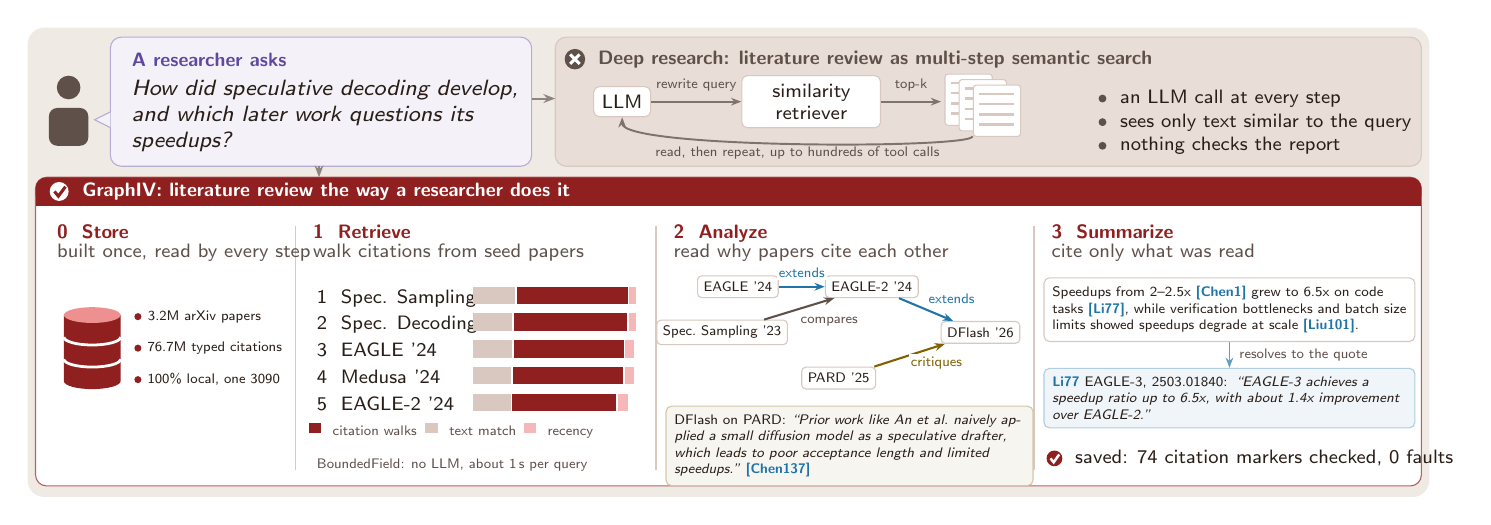
\begin{tikzpicture}[
  font=\sffamily\scriptsize,
  ink/.style={text=inkc},
  muted/.style={text=mutedc},
  row/.style={anchor=west, text=inkc, text height=1.6ex, text depth=0.3ex},
  stephead/.style={anchor=north west, align=left, font=\sffamily\scriptsize\bfseries, text=akred},
  paper/.style={draw=outlinec, rounded corners=1.5pt, fill=white, inner sep=2.2pt, font=\sffamily\tiny, text=inkc},
  edge/.style={-{Stealth[length=1.3mm]}, line width=0.75pt},
  intent/.style={font=\sffamily\tiny, fill=white, inner sep=0.8pt},
  box/.style={draw=outlinec, rounded corners=2pt, fill=white, inner sep=3pt, font=\sffamily\scriptsize, text=inkc, align=center},
  loop/.style={-{Stealth[length=1.3mm]}, mutedc!80, line width=0.7pt},
  feed/.style={-{Stealth[length=1.5mm]}, mutedc!70, line width=0.7pt},
  bullet/.style={anchor=north west, text width=1.75cm, align=left, font=\sffamily\tiny, text=inkc, inner sep=0pt},
]
\definecolor{akred}{HTML}{902020}
\definecolor{akredlight}{HTML}{E86060}
\definecolor{blueink}{HTML}{1F74A8}
\definecolor{ochreink}{HTML}{806000}
\definecolor{purpleink}{HTML}{6048A0}
\definecolor{inkc}{HTML}{2A1E18}
\definecolor{mutedc}{HTML}{60504A}
\definecolor{outlinec}{HTML}{D8C8C0}
\definecolor{paperc}{HTML}{F0EAE4}
\colorlet{cites}{akred}
\colorlet{textmatch}{outlinec}
\colorlet{recent}{akredlight!45!white}

\fill[paperc, rounded corners=6pt] (-0.1,0.66) rectangle (17.7,6.62);

% the question
\fill[mutedc] (0.42,5.86) circle (0.15);
\fill[mutedc, rounded corners=3pt] (0.17,5.12) rectangle (0.67,5.6);
\draw[draw=purpleink!45, fill=purpleink!7!white, rounded corners=4pt] (0.95,4.86) rectangle (6.3,6.5);
\draw[draw=purpleink!45, fill=purpleink!7!white] (0.95,5.55) -- (0.75,5.45) -- (0.95,5.35);
\fill[purpleink!7!white] (0.96,5.56) rectangle (1.0,5.34);
\node[anchor=north west, font=\sffamily\scriptsize\bfseries, text=purpleink] at (1.1,6.42) {A researcher asks};
\node[anchor=north west, text width=5cm, align=left, ink, font=\sffamily\footnotesize\itshape] at (1.1,6.08) {How did speculative decoding develop, and which later work questions its speedups?};

% deep research, the framing GraphIV departs from
\draw[draw=outlinec, fill=outlinec!35!paperc, rounded corners=4pt] (6.6,4.86) rectangle (17.6,6.5);
\fill[mutedc] (6.85,6.22) circle (0.13);
\draw[white, line width=1.1pt] (6.79,6.16) -- (6.91,6.28) (6.79,6.28) -- (6.91,6.16);
\node[anchor=west, font=\sffamily\scriptsize\bfseries, text=mutedc] at (7.02,6.22) {Deep research: literature review as multi-step semantic search};
\node[box] (llm) at (7.45,5.68) {LLM};
\node[box, text width=1.55cm] (ret) at (9.85,5.68) {similarity retriever};
\foreach \i in {0,1,2} {
  \draw[draw=outlinec, fill=white, rounded corners=1pt] (11.55+\i*0.18,5.38-\i*0.07) rectangle (12.15+\i*0.18,6.03-\i*0.07);
  \foreach \l in {0,1,2,3} \draw[outlinec, line width=0.9pt] (11.62+\i*0.18,5.92-\i*0.07-\l*0.13) -- (12.06+\i*0.18,5.92-\i*0.07-\l*0.13);
}
\draw[loop] (llm) -- node[above, muted, font=\sffamily\tiny] {rewrite query} (ret);
\draw[loop] (ret) -- node[above, muted, font=\sffamily\tiny] {top-k} (11.5,5.68);
\draw[loop] (11.9,5.24) .. controls (11.9,5.08) and (7.45,5.08) .. node[pos=0.5, below=0pt, muted, font=\sffamily\tiny, inner sep=1pt] {read, then repeat, up to hundreds of tool calls} (llm.south);
\foreach \t [count=\k] in {an LLM call at every step, sees only text similar to the query, nothing checks the report} {
  \fill[mutedc] (13.55,6.02-\k*0.3) circle (0.05);
  \node[anchor=west, ink] at (13.65,6.02-\k*0.3) {\t};
}

% GraphIV, the way a researcher does it
\draw[draw=akred!70, fill=white, rounded corners=4pt] (0,0.8) rectangle (17.6,4.72);
\fill[akred, rounded corners=4pt] (0,4.36) rectangle (17.6,4.72);
\fill[akred] (0,4.36) rectangle (17.6,4.5);
\fill[white] (0.3,4.54) circle (0.12);
\draw[akred, line width=1.1pt] (0.24,4.54) -- (0.29,4.48) -- (0.38,4.6);
\node[anchor=west, font=\sffamily\scriptsize\bfseries, text=white] at (0.47,4.54) {GraphIV: literature review the way a researcher does it};
\foreach \x in {3.3,7.88,12.68} \draw[outlinec] (\x,1.0) -- (\x,4.1);

\node[stephead] at (0.15,4.24) {0\ \ Store\\[-1pt]\textmd{\textcolor{mutedc}{built once, read by every step}}};
\begin{scope}[shift={(0.72,2.55)}]
  \fill[akred] (-0.36,0.42) -- (-0.36,-0.42) arc[start angle=180, end angle=360, x radius=0.36, y radius=0.1] -- (0.36,0.42) -- cycle;
  \fill[akredlight!70!white] (0,0.42) ellipse[x radius=0.36, y radius=0.1];
  \foreach \y in {0.14,-0.14} \draw[white, line width=1pt] (-0.36,\y) arc[start angle=180, end angle=360, x radius=0.36, y radius=0.1];
\end{scope}
\foreach \t/\y in {3.2M arXiv papers/2.95, {76.7M typed citations}/2.55, {100\% local, one 3090}/2.15} {
  \fill[akred] (1.3,\y) circle (0.045);
  \node[anchor=west, text width=1.8cm, align=left, font=\sffamily\tiny, text=inkc, inner sep=0pt] at (1.42,\y) {\t};
}

\node[stephead] at (3.4,4.24) {1\ \ Retrieve\\[-1pt]\textmd{\textcolor{mutedc}{walk citations from seed papers}}};
\node[row] at (3.45,3.22) {1\ \ Spec. Sampling '23};
\fill[textmatch] (5.550,3.11) rectangle (6.092,3.33);
\fill[cites] (6.112,3.11) rectangle (7.521,3.33);
\fill[recent] (7.541,3.11) rectangle (7.630,3.33);
\node[row] at (3.45,2.88) {2\ \ Spec. Decoding '22};
\fill[textmatch] (5.550,2.77) rectangle (6.053,2.99);
\fill[cites] (6.073,2.77) rectangle (7.515,2.99);
\fill[recent] (7.535,2.77) rectangle (7.621,2.99);
\node[row] at (3.45,2.54) {3\ \ EAGLE '24};
\fill[textmatch] (5.550,2.43) rectangle (6.055,2.65);
\fill[cites] (6.075,2.43) rectangle (7.468,2.65);
\fill[recent] (7.488,2.43) rectangle (7.602,2.65);
\node[row] at (3.45,2.20) {4\ \ Medusa '24};
\fill[textmatch] (5.550,2.09) rectangle (6.040,2.31);
\fill[cites] (6.060,2.09) rectangle (7.462,2.31);
\fill[recent] (7.482,2.09) rectangle (7.596,2.31);
\node[row] at (3.45,1.86) {5\ \ EAGLE-2 '24};
\fill[textmatch] (5.550,1.75) rectangle (6.032,1.97);
\fill[cites] (6.052,1.75) rectangle (7.373,1.97);
\fill[recent] (7.393,1.75) rectangle (7.522,1.97);
\fill[cites] (3.47,1.47) rectangle (3.63,1.6); \node[row, muted, font=\sffamily\tiny] at (3.65,1.535) {citation walks};
\fill[textmatch] (4.95,1.47) rectangle (5.11,1.6); \node[row, muted, font=\sffamily\tiny] at (5.13,1.535) {text match};
\fill[recent] (6.2,1.47) rectangle (6.36,1.6); \node[row, muted, font=\sffamily\tiny] at (6.38,1.535) {recency};
\node[row, muted, font=\sffamily\tiny] at (3.45,1.12) {BoundedField: no LLM, about 1\,s per query};

\node[stephead] at (7.98,4.24) {2\ \ Analyze\\[-1pt]\textmd{\textcolor{mutedc}{read why papers cite each other}}};
\node[paper] (sps) at (8.72,2.75) {Spec.\ Sampling '23};
\node[paper] (eagle) at (8.92,3.33) {EAGLE '24};
\node[paper] (eagle2) at (10.62,3.33) {EAGLE-2 '24};
\node[paper] (pard) at (10.2,2.17) {PARD '25};
\node[paper] (dflash) at (12.0,2.75) {DFlash '26};
\draw[edge, blueink] (eagle) -- node[intent, text=blueink, above=2pt] {extends} (eagle2);
\draw[edge, mutedc] (sps) -- node[intent, text=mutedc, pos=0.42, below right=2pt] {compares} (eagle2);
\draw[edge, blueink] (eagle2) -- node[intent, text=blueink, pos=0.45, above right=1pt] {extends} (dflash);
\draw[edge, ochreink] (pard) -- node[intent, text=ochreink, below right=-1pt] {critiques} (dflash);
\node[anchor=north west, text width=4.45cm, align=left, ink, font=\sffamily\tiny, fill=ochreink!6!white, draw=ochreink!35, rounded corners=2pt, inner sep=3pt] at (8.0,1.82) {DFlash on PARD: \itshape ``Prior work like An et al.\ naively applied a small diffusion model as a speculative drafter, which leads to poor acceptance length and limited speedups.''\upshape\ \textcolor{blueink}{\textbf{[Chen137]}}};

\node[stephead] at (12.78,4.24) {3\ \ Summarize\\[-1pt]\textmd{\textcolor{mutedc}{cite only what was read}}};
\node[anchor=north west, text width=4.5cm, align=left, ink, font=\sffamily\tiny, draw=outlinec, fill=white, rounded corners=2pt, inner sep=3pt] (report) at (12.8,3.45) {Speedups from 2--2.5x \textcolor{blueink}{\textbf{[Chen1]}} grew to 6.5x on code tasks \textcolor{blueink}{\textbf{[Li77]}}, while verification bottlenecks and batch size limits showed speedups degrade at scale \textcolor{blueink}{\textbf{[Liu101]}}.};
\node[anchor=north west, text width=4.5cm, align=left, ink, font=\sffamily\tiny, fill=blueink!7!white, draw=blueink!35, rounded corners=2pt, inner sep=3pt] (li77) at (12.8,2.3) {\textcolor{blueink}{\textbf{Li77}} EAGLE-3, 2503.01840: \itshape ``EAGLE-3 achieves a speedup ratio up to 6.5x, with about 1.4x improvement over EAGLE-2.''};
\draw[-{Stealth[length=1.3mm]}, blueink!70, line width=0.6pt] (report.south) -- node[right, muted, font=\sffamily\tiny] {resolves to the quote} (li77.north);
\fill[akred] (12.94,1.15) circle (0.1);
\draw[white, line width=0.9pt] (12.89,1.15) -- (12.93,1.1) -- (13.0,1.2);
\node[anchor=west, ink] at (13.08,1.15) {saved: 74 citation markers checked, 0 faults};

% the question feeds both
\draw[feed] (3.6,4.86) -- (3.6,4.72);
\draw[feed] (6.3,5.72) -- (6.6,5.72);
\end{tikzpicture}

\Description{A question about speculative decoding feeds two panels. The upper panel, in gray, shows deep research as a loop between an LLM and a similarity retriever. The lower panel, in red, shows GraphIV in four steps: a database of 3.2M arXiv papers and 76.7M typed citations built once and run locally; a ranked list of five papers with score bars mostly from citation walks; a small graph of five papers joined by edges labeled extends, compares and critiques with one citing sentence quoted; and a report excerpt whose label resolves to the quote it rests on, with 74 citation markers checked and 0 faults.}
\caption{GraphIV reviews literature the way a researcher does. Top: typical deep research agent treat literature as multi-step semantic search. Bottom: GraphIV approaches the same qieru from a citatiopn graph. BoundedField walks citations from the papers most similar to the question with no LLM/ \texttt{list\_citations} and \texttt{trace\_lineages} explains why each paper cites another, and \texttt{save\_report} saves the report only after all quotes are mechanically checked.}
\label{fig:teaser}
\end{teaserfigure}

\maketitle

\section{Introduction}
\label{sec:introduction}

Literature review is a crucial process of research. Successful literature review hinges on the ability to understand the field's landscape, present and past, and examine how the ideas are interconnected. This process can be broken down into sub-steps: retrieval (finding the right literature), analysis (understanding the connections between these papers), and summary (the synthesis of ideas and claims rooted in the source literature). The manual process is long and laborious; it begins with a few seed papers (often reviews), followed by the process of tracing citations to expand the list, and reading abstracts to decide which papers to read in full. An experienced reader needs about an hour to understand a single paper \citep{keshav2007read}, while a review on arXiv cites a median of 149 other arXiv papers and a systematic review takes 67 weeks on average \citep{huotala2024screening}.

Existing systems attempt to automate this process as search over text. Lexical and embedding retrievers are designed to retrieve literature based on term or semantic similarity \citep{robertson2009bm25,singh2022scirepeval,ostendorff2022scincl}. Deep research agents simply wrap these retrievers in a loop, where an LLM invokes queries over multiple turns \citep{he2025pasa,tongyi2025deepresearch,li2025webthinker,mirothinker2025}, treating literature review as a multi-step semantic search problem. This introduces a bottleneck reported by ScholarCatalyst \citep{kim2026scholarcatalyst}: each call queries the corpus through the same similarity retriever's top results, so repeated querying alone cannot improve over the retriever.

We argue that literature review is not simply a semantic search problem. Building on the manual process of tracing citations, systems like PaSa \citep{he2025pasa} and SciRAG \citep{ding2025scirag} attempted to leverage the citation graph in automated literature review. However, both systems incur an LLM invocation at every step for retrieval; PaSa has an LLM decide on which section's references to expand, while SciRAG uses GPT-4o to walk the citation graph. As each repeated query and citation hop invokes an LLM call, the cost of deep research systems grows quickly with the size of the query, with open agents now running up to 600 tool calls per question \citep{mirothinker2025}, at high inference cost and latency \citep{chen2026searchmore}. Yet a citation records what a field chose to read, and once the graph is built, following it needs no LLM at all.

We therefore introduce \textbf{BoundedField}, an LLM-free and citation-aware retriever that ranks papers the way a researcher reviews them, and that enhances the recall of any off-the-shelf embedding model it runs on. BoundedField takes the papers most similar to the question as a core, expands them by one citation hop, and scores each candidate as a product of bounded terms, $\prod_t (1+x_t)^{w_t}$, that measure how the core's citations reach it, along with its text match and recency. Each term lies on $[0,1]$, so a signal a paper lacks, such as citations to a paper too new to be cited, leaves its score unchanged rather than zeroing it. The exponents $w_t$ are the whole recipe: adapting BoundedField to a new task means fitting a handful of numbers on its training split, with no model trained and no LLM called, and a query takes about one second.

BoundedField runs on GraphIV, a citation graph of arXiv we computed once from arXiv's open HTML renders (3.2 million papers and 76.7 million resolved citations, growing), with each citation labeled with one of six intents and each paper with its probability of being a review. Unlike other scholarly citation graphs, which are either unfree or infrequently updated \citep{kinney2023s2,priem2022openalex,saier2023unarxive}, GraphIV is free and updates biweekly. To measure retrieval against real historical reviews, we mined three benchmarks from GraphIV's reviews, whose answer keys are reference lists that researchers wrote: SurveyMatch asks what a review cites, FrontierMatch asks for the papers the later of two reviews on the same topic cites and the earlier does not, and ConsensusMatch asks what several reviews of a topic all cite.

On these three benchmarks and five existing ones from PaSa, SurGE, and ScholarCatalyst, BoundedField led BM25, dense retrievers, a reranker, and two graph baselines at every recall cutoff but one. It more than doubled the recall of cosine search over the same embedder on all three of our benchmarks, from 0.087 to 0.216 at R@100 on SurveyMatch and from 0.257 to 0.731 on ConsensusMatch, and it beat PPR, the strongest baseline, by 51\% on SurveyMatch and 84\% on FrontierMatch. The gain comes from the graph rather than the embedder: on our three benchmarks and SurGE, BoundedField over a 475M-parameter embedder outperformed cosine search with each of seven larger embedders, up to 27B parameters \citep{zhang2025qwen3embedding,microsoft2026harrier,nvidia2026nemotronembed}. As one use of BoundedField, GraphIV-MCP gives an open-weight 27B agent six tools to search, read, and trace citations, and the agent may cite only quotes it has read (\cref{fig:teaser}). It finished all 63 report runs on a Ryzen 7 7700X and an RTX 3090 with no paid API call, at 12.7 minutes for a standard report.

Our results suggest that retrieval for literature review is better served by following what a field cites than by searching its text, and that built this way, automated literature review needs nothing more than consumer hardware. We release the graph, the benchmarks, the classifiers, and the code as a first step toward an open web of science.\footnote{\furl{https://huggingface.co/kkuroma} and \furl{https://git.kuroma.dev/kkuroma/graphiv}}

\section{Related Work}
\label{sec:related}

\subsection{Open Citation Datasets}
S2ORC released 81.1 million papers with resolved references \citep{lo2020s2orc}, and the Semantic Scholar Open Data Platform labels intents with the three-class SciCite model, though its bulk datasets require an API key \citep{kinney2023s2,cohan2019scaffolds}. OpenAlex updates quarterly \citep{priem2022openalex}, and OpenCitations releases resolved references without their contexts \citep{peroni2019opencitations}. Closest to ours, unarXive structured 1.9 million arXiv papers, of which only 165k are freely available \citep{saier2023unarxive}. Unlike these, GraphIV is free, updates biweekly, and labels why each citation was made.

\subsection{Literature Retrieval Benchmarks}
Most literature retrieval benchmarks pair a query with a few known papers. LitSearch holds 597 queries \citep{ajith2024litsearch}, and PaSa built 35k synthetic queries plus 50 real ones in RealScholarQuery \citep{he2025pasa}. Others rely on human annotation, which limits their scale: SPARBench holds 50 queries \citep{shi2025spar}, and ScholarCatalyst asked 184 authors which prior work advanced their projects \citep{kim2026scholarcatalyst}. SurGE, closest to ours, scores recall of 205 surveys' reference lists \citep{su2025surge}, but its surveys are fixed at release, while ours grow with every update.

\subsection{Citation-Aware Retrieval}
Most literature retrievers rank papers by text alone. BM25 matches terms \citep{robertson2009bm25}, while SPECTER2 and SciNCL use citations only to train their embeddings \citep{singh2022scirepeval,ostendorff2022scincl}. OpenScholar, PaperQA, and LitLLM retrieve densely before reranking or reading with an LLM \citep{asai2024openscholar,lala2023paperqa,agarwal2024litllm}, and so inherit the same first pool, which ScholarCatalyst found repeated querying cannot improve on \citep{kim2026scholarcatalyst}. Systems that follow citations at query time pay for every hop: PaSa has an LLM decide which section's references to expand \citep{he2025pasa}, SciRAG uses GPT-4o to walk the citation graph \citep{ding2025scirag}, and Crase and StructSurvey have agents fetch citation links from a hosted API, with Crase expanding 1.5 hops through Semantic Scholar over 500k arXiv papers \citep{hazra2026crase,pedinotti2026structsurvey}. Graph methods without an LLM fold the graph into a single signal: Personalized PageRank propagates one score from the seed papers \citep{page1999pagerank}, and GAR uses corpus graph neighbors only to fill the pool a neural reranker orders \citep{macavaney2022gar}. BoundedField differs on three counts. It walks a graph computed once rather than fetched per question, it scores what the core cites, what cites the core, and what is cited alongside it as separate bounded terms, and it fits a weight per term for each task, so it needs no model beyond the initial embedding and no LLM at any step.

\subsection{Automated Research Agents}
Deep research agents loop over search, reading, and writing a report, such as Tongyi DeepResearch \citep{tongyi2025deepresearch} and WebThinker \citep{li2025webthinker}, with MiroThinker running up to 600 tool calls per question \citep{mirothinker2025}. Their reports are not reliably grounded: DeepTRACE found 97.5\% unsupported statements in Perplexity's Deep Research \citep{venkit2025deeptrace}, and 3\% to 13\% of citation URLs from commercial systems were hallucinated \citep{rao2026hallucinations}. GraphIV-MCP lets its agent cite only quotes it has read, which the server confirms by string matching before saving a report.

\section{Method}
\label{sec:method}

We introduce GraphIV (Graph + arXiv), an open citation intent graph of arXiv, alongside BoundedField, a tunable, LLM-free, citation-aware retriever, and GraphIV-MCP, a suite of research tools. To keep GraphIV self-hostable, everything was built and tested on one consumer machine: an AMD Ryzen 7 7700X, 64 GB of memory, and an NVIDIA RTX 3090.

\subsection{Dataset}
\label{sec:dataset}

\begin{figure*}[t]
\centering
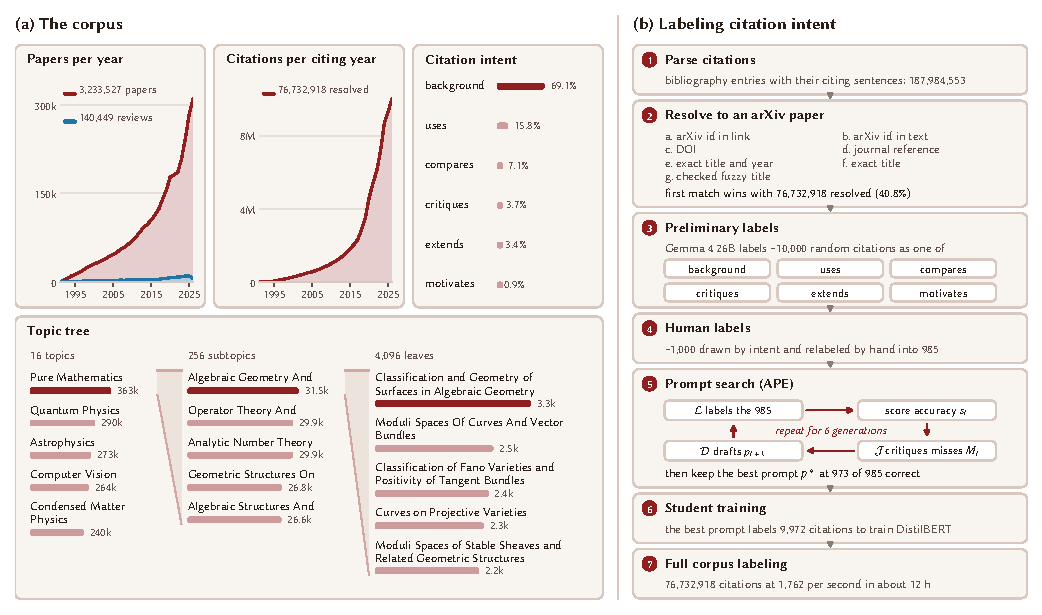
\includegraphics[width=\textwidth]{figures/dataset.pdf}
\Description{Two panels. Panel (a), the corpus, has four charts. Papers per year rises from near zero in the early 1990s to about 300 thousand a year by 2025, for 3,233,527 papers, with reviews a thin line below it totaling 140,449. Resolved citations per citing year rise steeply after 2015 to 76,732,918 in all. Citation intent is a bar chart: background 69.1\%, uses 15.8\%, compares 7.1\%, critiques 3.7\%, extends 3.4\%, motivates 0.9\%. The topic tree shows 16 topics, led by Pure Mathematics with 363 thousand papers, then Quantum Physics, Astrophysics, Computer Vision, and Condensed Matter Physics; 256 subtopics, led by Algebraic Geometry with 31.5 thousand; and 4,096 leaves, led by classification and geometry of surfaces in algebraic geometry with 3.3 thousand. Panel (b), labeling citation intent, is a seven-step pipeline from top to bottom: parse 187,984,553 citations with their citing sentences; resolve each to an arXiv paper by seven strategies in order, the first match winning, resolving 76,732,918 (40.8\%); Gemma 4 26B labels about 10,000 random citations as one of six intents; about 1,000 drawn by intent are relabeled by hand into 985; a prompt search loop in which the labeler labels the 985, the accuracy is scored, the judge critiques the misses, and the drafter writes the next prompt, repeated for six generations, keeping the best prompt at 973 of 985 correct; the best prompt labels 9,972 citations to train a DistilBERT student; and the student labels all 76,732,918 citations at 1,762 per second in about 12 hours.}
\caption{GraphIV's overview. (a) The corpus as broken down per year alongside its citation intent and topic tree. (b) The citation intent labeling pipeline, in which the labeler $\mathcal{L}$, judge $\mathcal{J}$, and drafter $\mathcal{D}$ search for the teacher prompt.}
\label{fig:dataset}
\end{figure*}

GraphIV was built from Cornell's arXiv metadata snapshot on Kaggle \citep{clement2019arxiv}, which is free and updated biweekly. Each alternative misses one of these: Semantic Scholar's bulk datasets require an API key\footnote{\furl{https://semanticscholar.org/product/api}} \citep{kinney2023s2}, OpenAlex's free snapshot is quarterly and its daily one paid\footnote{\furl{https://help.openalex.org/access/pricing}} \citep{priem2022openalex}, and unarXive, the closest predecessor, is frozen at 2022 \citep{saier2023unarxive}. As the snapshot holds only per-paper metadata, we built the citation graph from arXiv's open HTML renders. As of 2026-11-11, the corpus held 3,233,527 papers, 3,196,302 of them processed.

\paragraph{Citation extraction and resolution:}
For each paper with an HTML version, we parsed its bibliography and the sentences citing each entry. As arXiv bibliographies follow no single convention, we resolved citations with the strategies in \cref{tab:resolution}. Of 187,984,553 parsed citations, 76,732,918 (40.8\%) resolved to a paper in the corpus.

\begin{table}[t]
\caption{Citation resolution strategies. Numbers shown correspond to additional citations resolved after a method is employed.}
\label{tab:resolution}
\centering
\small
\begin{tabular}{lr}
\toprule
Method & Citations \\
\midrule
arXiv id in the text & 21,831,361 \\
Exact title and year & 16,478,534 \\
Journal reference & 13,397,614 \\
arXiv id in the link & 10,058,637 \\
Fuzzy title & 8,491,441 \\
DOI & 4,108,520 \\
Exact title, year disagrees & 2,366,811 \\
\midrule
Resolved & 76,732,918 \\
Fuzzy match rejected & 18,253,288 \\
No match & 92,998,347 \\
\midrule
Parsed & 187,984,553 \\
\bottomrule
\end{tabular}
\end{table}

\paragraph{Citation intent:}
We classified each citation into one of six intents: \term{background}, \term{uses}, \term{compares}, \term{extends}, \term{critiques}, and \term{motivates}. Existing classifiers are coarser: SciCite uses background, method, and result comparison \citep{cohan2019scaffolds}, while ACL-ARC and MultiCite separate extending from comparing but fold critiques into comparison \citep{jurgens2018citation,lauscher2022multicite}. We kept \term{critiques} separate since, with \term{extends} and \term{compares}, it forms what our lineage tracing follows.

As labeling 76.7 million citations with an LLM on one GPU is not computationally realistic, we distilled one into a small classifier (\cref{fig:dataset}b). Gemma 4 26B \citep{gemmateam2026gemma4} labeled 10,000 random citations, from which a stratified sample of about 1,000 was relabeled by hand, leaving 985 human-labeled citations $\{(x_i, y_i)\}_{i=1}^{n}$. Against these, we ran automatic prompt engineering \citep{zhou2023ape}: at generation $t$, the labeler $\mathcal{L}$ labeled every citation under prompt $p_t$, the judge $\mathcal{J}$ critiqued $p_t$ from its misses alone, and the drafter $\mathcal{D}$ wrote the next prompt from the critique (\cref{eq:ape}).
\begin{equation}
    \label{eq:ape}
    \begin{aligned}
        \hat{y}_{i,t} &= \mathcal{L}(x_i, p_t) && \text{labeler} \\
        s_t &= \frac{1}{n} \sum_{i=1}^{n} \mathbb{1}\left[\hat{y}_{i,t} = y_i\right] && \text{score} \\
        c_t &= \mathcal{J}\left(p_t, \left\{(x_i, y_i, \hat{y}_{i,t}) : \hat{y}_{i,t} \neq y_i\right\}\right) && \text{judge} \\
        p_{t+1} &= \mathcal{D}(p_t, c_t) && \text{drafter} \\
        p^{\ast} &= p_{\operatorname*{arg\,max}_{t} s_t} && \text{selection}
    \end{aligned}
\end{equation}

Unparsable replies counted as misses, and the judge saw at most 60 misses per generation. After six generations, $p^{\ast}$ labeled 973 of the 985 correctly, and then labeled about 10,000 fresh citations to train a DistilBERT student \citep{sanh2019distilbert} at an 8:1:1 split. The student agreed with the teacher at 0.886 accuracy and 0.815 macro F1 on the 998 test citations, and reached 0.981 macro F1 on the 985 human labels, which it never trained on, against the teacher's 0.988. At 1,762 citations per second on the 3090, it labeled the corpus in 12 hours.

\paragraph{Survey detection:}
Reviews' reference lists are the answer keys of our benchmarks (\cref{sec:benchmarks}). A title regex over ``survey'', ``review'', and nine other words reached a recall of 0.185 at 0.409 precision, as 81\% of reviews carry none of them. Instead, a second DistilBERT read the title and abstract, trained on 24,000 papers labeled by Gemma 4 26B, half with a review word in the title. It reached 0.878 average precision against the LLM labels, and 140,449 papers scored above 0.5.

\paragraph{Embeddings:}
By default, every title and abstract was embedded by nomic-embed-text-v2-moe (Nomic) \citep{nussbaum2025moe} into 768 dimensions, truncated to 512 tokens, at 185 papers per second, or 5 hours for the corpus. The embedder is off the shelf by design, so it can be swapped: the 3,186,931 papers of the 2026-10-01 release were also embedded with seven open embedders from 0.6B to 27B parameters, Qwen3-Embedding (Qwen3) 0.6B, 4B, and 8B \citep{zhang2025qwen3embedding}, Harrier-OSS-v1 (Harrier) 0.6B and 27B \citep{microsoft2026harrier}, and Nemotron-3-Embed (Nemotron) 1B and 8B \citep{nvidia2026nemotronembed}, each with its own document and query prompts (\cref{sec:embedders}).

\paragraph{Topic tree:}
We projected each embedding to 50 dimensions with UMAP \citep{mcinnes2018umap} and clustered with $k$-means \citep{lloyd1982kmeans} three times at $k=16$, giving 16 topics, 256 subtopics, and 4,096 leaves. Gemma 4 26B named each node from the ten children, or papers for a leaf, nearest its centroid.

\subsection{Benchmarks}
\label{sec:benchmarks}

We evaluated retrieval on five existing benchmarks from three sources and three of our own, capping every case at the date its answer key was drawn. We report R@$k$, the share of a case's answers among the top $k$ papers returned, and nDCG@$k$ where a benchmark's authors report it.

\subsubsection{Existing Benchmarks}
We used PaSa's AutoScholarQuery (29,886 train, 901 validation, and 899 test queries) and RealScholarQuery (49 queries) \citep{he2025pasa}, keeping queries whose answers are all in GraphIV. SurGE carries no arXiv ids, so we matched its papers by title, leaving 193 surveys \citep{su2025surge}. ScholarCatalyst's 207 core and 687 subfield queries were scored inside its own corpus \citep{kim2026scholarcatalyst}. Each benchmark was scored at its published $k$.

\begin{figure*}[t]
\centering
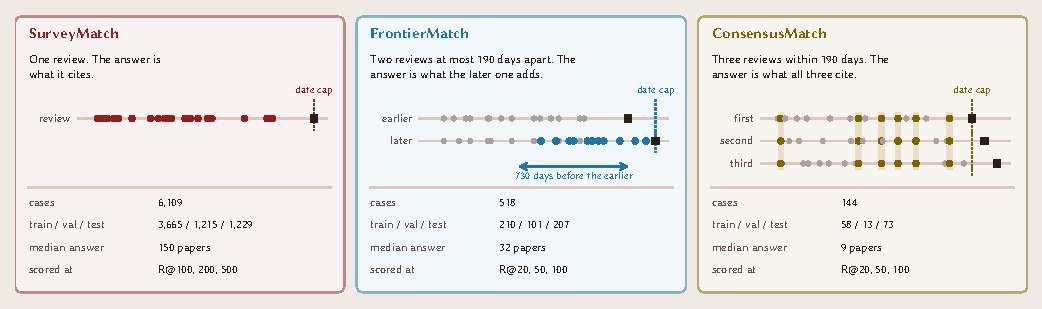
\includegraphics[width=\textwidth]{figures/benchmarks.pdf}
\Description{Three cards, one per benchmark, each with a timeline schematic and a table of counts. SurveyMatch: one review, whose references are all colored as the answer, with the date cap at the review; 6,109 cases split 3,665 train, 1,215 validation, 1,229 test; a median answer of 150 papers; scored at R@100, 200, and 500. FrontierMatch: two reviews at most 190 days apart, an earlier and a later one, where only the references the later one adds are colored, the date cap sits at the earlier review, and an arrow marks the 730 days before it; 518 cases split 210, 101, 207; a median answer of 32 papers; scored at R@20, 50, and 100. ConsensusMatch: three reviews within 190 days, where only the references all three share are colored and joined by vertical bands, with the date cap before the reviews; 144 cases split 58, 13, 73; a median answer of 9 papers; scored at R@20, 50, and 100.}
\caption{The proposed benchmarks. Each row is one review on a timeline with its references as dots, the answer in color, and the date cap the retriever is held to. The schematics are illustrative and the counts are from the 2026-10-22 release.}
\label{fig:benchmarks}
\end{figure*}

\subsubsection{Proposed Benchmarks}

Existing benchmarks fall short of real literature research in three ways: most pair a query with a few papers while a review cites over 100, their keys are chosen by annotators or LLMs rather than by researchers for their own work, and each case comes from a single source paper. We addressed all three by mining benchmarks from GraphIV's own reviews (\cref{fig:benchmarks}), whose reference lists are large keys written by researchers. The topic tree and the survey classifier also let us group several reviews of one topic into a case, which to our knowledge no existing benchmark does, to ask what a field added over time and what it agrees on.

A review is a paper with a survey probability of at least 0.95, where the classifier's precision is 0.937, and its references are the papers it cites that resolved in GraphIV and predate it. Gemma 4 26B wrote each case's research question from the titles, frozen in the release.

\begin{itemize}
    \item \textbf{SurveyMatch} asks what a review cites. A case is one review with at least 100 references, which are its answers.
    \item \textbf{FrontierMatch} asks what a field picked up over a short period. A case is two reviews in one topic leaf, at most 190 days apart with a cosine of at least 0.80, and its answers are what the later review cites and the earlier does not, dated at most 730 days before the earlier one.
    \item \textbf{ConsensusMatch} asks what every review of a topic agrees on. A case is three reviews in one leaf within 190 days, each pair at a cosine of at least 0.75, and its answers are what all three cite.
\end{itemize}

We split cases by hashing their anchors' arXiv ids, so a newer release is strictly additive. SurveyMatch is scored at R@100, 200, and 500, and the smaller FrontierMatch and ConsensusMatch at R@20, 50, and 100.

\subsection{Retrieval (BoundedField)}
\label{sec:bf}

BoundedField is an LLM-free, citation-aware retriever. Given a question, it retrieves the 5,000 papers most cosine-similar to it, dated on or before its cap. The top 200 form the \term{core}, and expanding the list by one citation hop to and from the core gives the \term{pool}.

\paragraph{Walking the citation graph:}
Let $A \in \{0,1\}^{|P| \times |P|}$ be the citation graph on the \term{pool} $P$, where $A_{ij} = 1$ if paper $j$ cites paper $i$, and $c\in\mathbb{R}^{|P|}$ the core's cosines, zero elsewhere, normalized to sum to one. Multiplying by $A$ walks one hop back in time and by $A^\top$ one hop forward, so graph traversal reduces to matrix products. Each walk gives a raw term $u_\tau \in \mathbb{R}_{\geq 0}^{|P|}$:
\begin{equation}
    \label{eq:walks}
    \begin{aligned}
        u_{\text{anc}} &= A c, & u_{\text{fro}} &= A^\top c, & u_{\text{cocite}} &= (A A^\top c) \odot r, \\
        u_{\text{anc2}} &= A^2 c, & u_{\text{fro2}} &= (A^\top)^2 c, & u_{\text{couple}} &= (A^\top A c) \odot r.
    \end{aligned}
\end{equation}
$Ac$ is what the core cites, $A^\top c$ what cites it, and $AA^\top c$ and $A^\top A c$ are co-citation \citep{small1973cocitation} and bibliographic coupling \citep{kessler1963coupling} seeded by the core, weighted by the recency $r_p = 1/(1+a_p)$ of a paper aged $a_p$ years at the cap. We write $W$ for these six walks.

\paragraph{Additional terms:}
BoundedField also scores the cosine $u_{\text{cos}}$, the recency $u_{\text{rec}} = r$, and the question's BM25 within the pool $u_{\text{bm25}}$ \citep{robertson2009bm25}. As $u_{\text{anc}}$ and $u_{\text{fro}}$ are zero beyond the core's direct neighbors, two decay terms $u_{\text{anc\_decay},p} = \delta^{d^{\leftarrow}(p)}$ and $u_{\text{fro\_decay},p} = \delta^{d^{\rightarrow}(p)}$, with $\delta = 0.5$, let farther papers score, where $d^{\leftarrow}(p)$ and $d^{\rightarrow}(p)$ are the fewest hops from the core walking $A$ and $A^\top$, up to 4, and the term is zero beyond. The hub term counts a paper's citations across all of GraphIV, $u_{\text{hub},p} = \sum_{j : t_j \leq t} \tilde{A}_{pj}$, for the full graph $\tilde{A}$, cap $t$, and paper dates $t_j$, excluding the case's anchors.

\paragraph{Bounding the terms:}
The raw terms are not comparable across queries: a walk grows with the size of the pool and the core, and its values are heavy-tailed, as a few landmark papers sit orders of magnitude above the rest. We therefore mapped every raw term $u_\tau$ to a bounded term $x_\tau \in [0,1]^{|P|}$, with a per-query normalization $N$ and, for the walks and hub, a compression $C_\lambda$:
\begin{gather*}
    N(v) = \frac{\max(v,0)}{\max_i \max(v_i,0)}, \\
    C_\lambda(v) = N\bigl(\log(1 + \lambda\,N(v))\bigr), \qquad \lambda = 100,
\end{gather*}
\begin{equation*}
    x_\tau =
    \begin{cases}
        C_\lambda(u_\tau) & \tau \in W \cup \{\text{hub}\}, \\
        u_\tau & \tau \in \{\text{anc\_decay}, \text{fro\_decay}\}, \\
        N(u_\tau) & \text{otherwise}.
    \end{cases}
\end{equation*}
$N$ is invariant to scale, $N(\alpha v) = N(v)$ for $\alpha > 0$, so a bounded term depends only on how the papers of one pool compare with each other. $C_\lambda$ preserves order and zeros and maps the top paper to 1, but lifts a paper at 1\% of the top from 0.01 to $\log 2 / \log 101 \approx 0.15$, so $\lambda$ sets how far below the top a term still separates papers. The decay terms already lie on $[0,1]$ and are left as they are. We then combined the bounded terms as a product of bounded factors:
\begin{equation}
    \label{eq:bf}
    \begin{aligned}
        \mathrm{score}(p) &= \frac{\prod_{\tau \in T} \left(1 + x_{\tau,p}\right)^{w_\tau}}{\left(1 + x_{\text{hub},p}\right)^{w_{\text{hub}}}}, \\
        \log \mathrm{score}(p) &= \sum_{\tau \in T} w_\tau \,\phi_{\tau,p} - w_{\text{hub}}\, \phi_{\text{hub},p},
    \end{aligned}
\end{equation}
where $T$ is every term but hub, $w_\tau \geq 0$, and $\phi_{\tau,p} = \log(1 + x_{\tau,p})$. This makes BoundedField fundamentally a linear ranking function over fixed, bounded features. A missing term is ignored (at 0 in the summation), meaning papers too new to be cited (with $x_{\text{anc}} = 0$) are not excluded. The exponents $w_\tau$ are what we tuned for each task (\cref{sec:tuning}).

\subsection{Automated Research System}
\label{sec:mcp}

GraphIV-MCP gives an LLM agent six tools over the Model Context Protocol \citep{anthropic2024mcp}, and the client owns the agent loop, turning the user's question into a sequence of calls. Our agent is an open-weight fine-tune of Qwen3.6 27B \citep{qwen2026qwen36}, served through llama.cpp \citep{gerganov2023llamacpp} on the same RTX 3090. The following tools are available:
\begin{itemize}
    \item \texttt{search\_papers} runs BoundedField with a specific recipe
    \item \texttt{recall\_paper} finds the one paper that best matches a description
    \item \texttt{read\_paper} answers a question about a paper in claims backed by verbatim quotes
    \item \texttt{list\_citations} returns a paper's citers or references with their intents and citing sentences
    \item \texttt{trace\_lineages} follows \term{extends}, \term{compares}, and \term{critiques} citations through a set of papers
    \item \texttt{save\_report} saves the report once every citation in it resolves to a quote the agent read
\end{itemize}
\Cref{app:agent} details each tool and the agent's effort presets, and \cref{app:questions} lists the 21 test questions.

% figures/embedders.pdf, its alt text and tables/recipes.tex are generated by benchmarks/scripts/results and copied by benchmarks/scripts/copy.sh
\begin{figure*}[t]
\centering
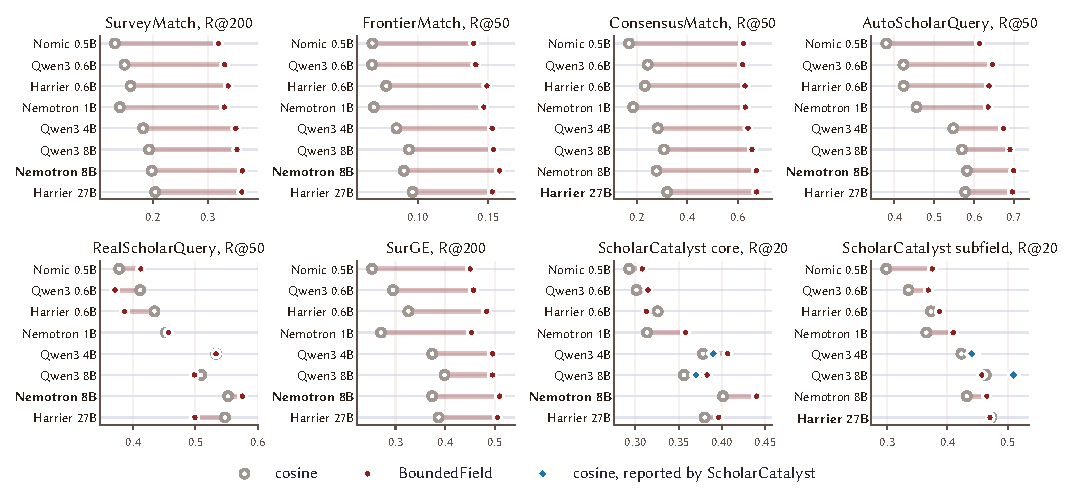
\includegraphics[width=\textwidth]{figures/embedders.pdf}
\Description{Eight dot-line panels in two rows, one per benchmark, each listing eight embedders from top to bottom by size: Nomic 0.5B, Qwen3 0.6B, Harrier 0.6B, Nemotron 1B, Qwen3 4B, Qwen3 8B, Nemotron 8B, Harrier 27B. Each row joins a hollow gray dot, recall with cosine search, an amber dot, recall with PPR, and a red dot, recall with BoundedField, and the embedder with the highest BoundedField recall in each panel is in bold. A star beside an embedder marks BoundedField significantly above its cosine search and a cross significantly above its PPR. On SurveyMatch, FrontierMatch, ConsensusMatch, AutoScholarQuery, SurGE, every BoundedField dot sits right of every cosine dot. On the two ScholarCatalyst panels, blue diamonds mark the cosine recall ScholarCatalyst reported for Qwen3 4B and 8B. Values, cosine to PPR to BoundedField, are: SurveyMatch at R@200: Nomic 0.5B 0.132 to 0.232 to 0.319; Qwen3 0.6B 0.149 to 0.249 to 0.331; Harrier 0.6B 0.160 to 0.252 to 0.337; Nemotron 1B 0.141 to 0.240 to 0.330; Qwen3 4B 0.183 to 0.278 to 0.350; Qwen3 8B 0.194 to 0.284 to 0.353; Nemotron 8B 0.198 to 0.295 to 0.363; Harrier 27B 0.205 to 0.290 to 0.361; best with BoundedField, Nemotron 8B. FrontierMatch at R@50: Nomic 0.5B 0.068 to 0.078 to 0.142; Qwen3 0.6B 0.068 to 0.079 to 0.139; Harrier 0.6B 0.078 to 0.089 to 0.145; Nemotron 1B 0.069 to 0.079 to 0.146; Qwen3 4B 0.085 to 0.097 to 0.152; Qwen3 8B 0.094 to 0.103 to 0.155; Nemotron 8B 0.090 to 0.099 to 0.159; Harrier 27B 0.096 to 0.094 to 0.153; best with BoundedField, Nemotron 8B. ConsensusMatch at R@50: Nomic 0.5B 0.170 to 0.470 to 0.607; Qwen3 0.6B 0.243 to 0.504 to 0.628; Harrier 0.6B 0.232 to 0.509 to 0.635; Nemotron 1B 0.185 to 0.502 to 0.627; Qwen3 4B 0.283 to 0.572 to 0.651; Qwen3 8B 0.308 to 0.599 to 0.662; Nemotron 8B 0.278 to 0.597 to 0.663; Harrier 27B 0.321 to 0.588 to 0.673; best with BoundedField, Harrier 27B. AutoScholarQuery at R@50: Nomic 0.5B 0.379 to 0.482 to 0.621; Qwen3 0.6B 0.423 to 0.527 to 0.646; Harrier 0.6B 0.423 to 0.521 to 0.641; Nemotron 1B 0.455 to 0.557 to 0.639; Qwen3 4B 0.548 to 0.632 to 0.690; Qwen3 8B 0.569 to 0.630 to 0.691; Nemotron 8B 0.582 to 0.663 to 0.702; Harrier 27B 0.578 to 0.634 to 0.694; best with BoundedField, Nemotron 8B. RealScholarQuery at R@50: Nomic 0.5B 0.377 to 0.404 to 0.374; Qwen3 0.6B 0.411 to 0.414 to 0.404; Harrier 0.6B 0.434 to 0.445 to 0.381; Nemotron 1B 0.453 to 0.444 to 0.425; Qwen3 4B 0.533 to 0.516 to 0.470; Qwen3 8B 0.509 to 0.499 to 0.493; Nemotron 8B 0.553 to 0.516 to 0.574; Harrier 27B 0.547 to 0.530 to 0.470; best with BoundedField, Nemotron 8B. SurGE at R@200: Nomic 0.5B 0.253 to 0.391 to 0.450; Qwen3 0.6B 0.295 to 0.405 to 0.458; Harrier 0.6B 0.326 to 0.425 to 0.479; Nemotron 1B 0.271 to 0.368 to 0.453; Qwen3 4B 0.374 to 0.453 to 0.487; Qwen3 8B 0.399 to 0.457 to 0.502; Nemotron 8B 0.374 to 0.475 to 0.508; Harrier 27B 0.387 to 0.453 to 0.507; best with BoundedField, Nemotron 8B. ScholarCatalyst core at R@20: Nomic 0.5B 0.293 to 0.304 to 0.289; Qwen3 0.6B 0.301 to 0.341 to 0.321; Harrier 0.6B 0.326 to 0.339 to 0.315; Nemotron 1B 0.314 to 0.333 to 0.326; Qwen3 4B 0.378 to 0.378 to 0.386; Qwen3 8B 0.356 to 0.377 to 0.375; Nemotron 8B 0.401 to 0.371 to 0.436; Harrier 27B 0.380 to 0.399 to 0.385; best with BoundedField, Nemotron 8B; reported cosine 0.39 for Qwen3 4B; reported cosine 0.37 for Qwen3 8B. ScholarCatalyst subfield at R@20: Nomic 0.5B 0.298 to 0.330 to 0.358; Qwen3 0.6B 0.335 to 0.370 to 0.387; Harrier 0.6B 0.373 to 0.405 to 0.377; Nemotron 1B 0.365 to 0.385 to 0.393; Qwen3 4B 0.423 to 0.442 to 0.432; Qwen3 8B 0.464 to 0.487 to 0.452; Nemotron 8B 0.432 to 0.431 to 0.466; Harrier 27B 0.473 to 0.492 to 0.463; best with BoundedField, Nemotron 8B; reported cosine 0.44 for Qwen3 4B; reported cosine 0.51 for Qwen3 8B.}

\caption{R@$k$ with cosine search, PPR, and BoundedField by embedder on all benchmarks, at each benchmark's middle cutoff. BoundedField runs used the recipe of each benchmark's mode, refit on each embedder: \term{survey} on SurveyMatch and SurGE, \term{frontier} and \term{consensus} on their own, and \term{focused} on PaSa and ScholarCatalyst. The embedding in bold has the highest BoundedField score. A star beside an embedder marks BoundedField significantly above its cosine search, and a cross significantly above its PPR, by a one-sided Wilcoxon signed-rank test on per-case recall, Holm-corrected over the 64 comparisons of each, $p < 0.05$. Diamond marks the cosine recall reported by ScholarCatalyst \cite{kim2026scholarcatalyst}.}
\label{fig:embedders}
\end{figure*}

% generated by benchmarks/scripts/results/table_main_recipes.py from benchmarks/data/runs/tune/nomic-focused_bf_seed0, benchmarks/data/runs/tune/nomic-survey_bf_seed0, benchmarks/data/runs/tune/nomic-frontier_bf_seed0, benchmarks/data/runs/tune/nomic-consensus_bf_seed0
\begin{table}[t]
\caption{The exponents of BoundedField's four recipes, with the benchmark and the R@$k$ each was tuned on.}
\label{tab:recipes}
\centering
\small
\setlength{\tabcolsep}{4pt}
\begin{tabular}{lrrrr}
\toprule
 & \term{focused} & \term{survey} & \term{frontier} & \term{consensus} \\
\midrule
\textbf{Source} & PaSa & SurveyMatch & FrontierMatch & ConsensusMatch \\
$k$ & 20 & 250 & 100 & 50 \\
\midrule
$w_{\text{cos}}$ & 1.00 & 1.00 & 1.00 & 1.00 \\
$w_{\text{rec}}$ & 0.45 & 0.95 & 0.85 & 1.59 \\
$w_{\text{bm25}}$ & 0.97 & 0.53 & 0.20 & 0.64 \\
$w_{\text{anc}}$ & 0.52 & 1.33 & 0.32 & 2.72 \\
$w_{\text{fro}}$ & 0.01 & 0.23 & 0.27 & 0.02 \\
$w_{\text{anc2}}$ & 0.13 & 0.26 & 0.00 & 0.08 \\
$w_{\text{fro2}}$ & 0.01 & 0.03 & 0.02 & 0.02 \\
$w_{\text{cocite}}$ & 0.50 & 1.98 & 1.35 & 0.19 \\
$w_{\text{couple}}$ & 0.06 & 0.02 & 0.01 & 0.02 \\
$w_{\text{anc\_decay}}$ & 0.01 & 0.02 & 0.05 & 0.06 \\
$w_{\text{fro\_decay}}$ & 0.01 & 0.02 & 0.01 & 0.02 \\
$w_{\text{hub}}$ & 0.01 & 0.23 & 4.23 & 0.06 \\
\bottomrule
\end{tabular}
\end{table}


% generated by paper/scripts/retrieval.py
% recall is recomputed from each run's rankings against benchmarks/data/cases/<benchmark>/<split>.jsonl, and ScholarCatalyst's nDCG and recall are the means of each run's per-case values
\begin{table*}[t]
\centering
\footnotesize
\setlength{\tabcolsep}{4pt}
\begin{subtable}{\textwidth}
\centering
\caption{The proposed benchmarks, test splits.}
\label{tab:proposed}
\begin{tabular}{lrrrrrrrrr}
\toprule
 & \multicolumn{3}{c}{SurveyMatch} & \multicolumn{3}{c}{FrontierMatch} & \multicolumn{3}{c}{ConsensusMatch} \\
\cmidrule(lr){2-4}\cmidrule(lr){5-7}\cmidrule(lr){8-10}
method & R@100 & R@200 & R@500 & R@20 & R@50 & R@100 & R@20 & R@50 & R@100 \\
\midrule
% benchmarks/data/runs/bm25-surveymatch.jsonl, benchmarks/data/runs/bm25-frontiermatch.jsonl, benchmarks/data/runs/bm25-consensusmatch.jsonl
BM25 & 0.066 & 0.100 & 0.162 & 0.027 & 0.051 & 0.080 & 0.058 & 0.113 & 0.167 \\
% benchmarks/data/runs/specter2-surveymatch.jsonl, benchmarks/data/runs/specter2-frontiermatch.jsonl, benchmarks/data/runs/specter2-consensusmatch.jsonl
SPECTER2 & 0.037 & 0.057 & 0.097 & 0.018 & 0.038 & 0.056 & 0.037 & 0.073 & 0.120 \\
% benchmarks/data/runs/scincl-surveymatch.jsonl, benchmarks/data/runs/scincl-frontiermatch.jsonl, benchmarks/data/runs/scincl-consensusmatch.jsonl
SciNCL & 0.059 & 0.093 & 0.158 & 0.023 & 0.047 & 0.077 & 0.082 & 0.148 & 0.233 \\
% benchmarks/data/runs/nomic_cosine-surveymatch.jsonl, benchmarks/data/runs/nomic_cosine-frontiermatch.jsonl, benchmarks/data/runs/nomic_cosine-consensusmatch.jsonl
Nomic cosine & 0.087 & 0.133 & 0.212 & 0.032 & 0.069 & 0.107 & 0.096 & 0.172 & 0.257 \\
% benchmarks/data/runs/rerank-surveymatch.jsonl, benchmarks/data/runs/rerank-frontiermatch.jsonl, benchmarks/data/runs/rerank-consensusmatch.jsonl
OpenScholar rerank & 0.083 & 0.130 & 0.217 & 0.028 & 0.055 & 0.093 & 0.070 & 0.151 & 0.220 \\
% benchmarks/data/runs/gar_sim-surveymatch.jsonl, benchmarks/data/runs/gar_sim-frontiermatch.jsonl, benchmarks/data/runs/gar_sim-consensusmatch.jsonl
GAR (similarity) & 0.085 & 0.135 & 0.235 & 0.029 & 0.056 & 0.094 & 0.073 & 0.159 & 0.238 \\
% benchmarks/data/runs/gar_cite-surveymatch.jsonl, benchmarks/data/runs/gar_cite-frontiermatch.jsonl, benchmarks/data/runs/gar_cite-consensusmatch.jsonl
GAR (citations) & 0.090 & 0.147 & 0.275 & 0.030 & 0.058 & 0.099 & 0.076 & 0.167 & 0.254 \\
% benchmarks/data/runs/ppr-surveymatch.jsonl, benchmarks/data/runs/ppr-frontiermatch.jsonl, benchmarks/data/runs/ppr-consensusmatch.jsonl
PPR & 0.143 & 0.229 & 0.375 & 0.028 & 0.077 & 0.122 & 0.274 & 0.441 & 0.556 \\
\midrule
% benchmarks/data/runs/survey-surveymatch.jsonl, benchmarks/data/runs/frontier-frontiermatch.jsonl, benchmarks/data/runs/consensus-consensusmatch.jsonl
BoundedField (Nomic) & 0.216 & 0.319 & 0.475 & 0.067 & 0.139 & 0.224 & 0.441 & 0.624 & 0.731 \\
% benchmarks/data/runs/bfrefit_nemotron_8b-surveymatch.jsonl, benchmarks/data/runs/bfrefit_nemotron_8b-frontiermatch.jsonl, benchmarks/data/runs/bfrefit_nemotron_8b-consensusmatch.jsonl
BoundedField (Nemotron 8B) & \textbf{0.246} & \textbf{0.363} & \textbf{0.529} & \textbf{0.073} & \textbf{0.158} & \textbf{0.244} & \textbf{0.488} & \textbf{0.673} & \textbf{0.797} \\
\bottomrule
\end{tabular}
\end{subtable}
\vspace{6pt}
\begin{subtable}{\textwidth}
\centering
\caption{PaSa's AutoScholarQuery test split and RealScholarQuery, and SurGE. PaSa's reported runs search Google rather than our corpus.}
\label{tab:existing}
\begin{tabular}{lrrrrrrrrr}
\toprule
 & \multicolumn{3}{c}{AutoScholarQuery} & \multicolumn{3}{c}{RealScholarQuery} & \multicolumn{3}{c}{SurGE} \\
\cmidrule(lr){2-4}\cmidrule(lr){5-7}\cmidrule(lr){8-10}
method & R@20 & R@50 & R@100 & R@20 & R@50 & R@100 & R@100 & R@200 & R@500 \\
\midrule
% benchmarks/data/runs/bm25-pasa_test.jsonl, benchmarks/data/runs/bm25-pasa_real.jsonl, benchmarks/data/runs/bm25-surge.jsonl
BM25 & 0.238 & 0.313 & 0.376 & 0.169 & 0.255 & 0.317 & 0.150 & 0.192 & 0.258 \\
% benchmarks/data/runs/specter2-pasa_test.jsonl, benchmarks/data/runs/specter2-pasa_real.jsonl, benchmarks/data/runs/specter2-surge.jsonl
SPECTER2 & 0.120 & 0.177 & 0.220 & 0.101 & 0.152 & 0.226 & 0.184 & 0.245 & 0.338 \\
% benchmarks/data/runs/scincl-pasa_test.jsonl, benchmarks/data/runs/scincl-pasa_real.jsonl, benchmarks/data/runs/scincl-surge.jsonl
SciNCL & 0.118 & 0.174 & 0.225 & 0.104 & 0.181 & 0.253 & 0.180 & 0.239 & 0.337 \\
% benchmarks/data/runs/nomic_cosine-pasa_test.jsonl, benchmarks/data/runs/nomic_cosine-pasa_real.jsonl, benchmarks/data/runs/nomic_cosine-surge.jsonl
Nomic cosine & 0.278 & 0.375 & 0.439 & 0.270 & 0.377 & 0.477 & 0.199 & 0.255 & 0.347 \\
% benchmarks/data/runs/rerank-pasa_test.jsonl, benchmarks/data/runs/rerank-pasa_real.jsonl, benchmarks/data/runs/rerank-surge.jsonl
OpenScholar rerank & 0.298 & 0.387 & 0.452 & 0.241 & 0.383 & 0.488 & 0.174 & 0.233 & 0.341 \\
% benchmarks/data/runs/gar_sim-pasa_test.jsonl, benchmarks/data/runs/gar_sim-pasa_real.jsonl, benchmarks/data/runs/gar_sim-surge.jsonl
GAR (similarity) & 0.299 & 0.391 & 0.463 & 0.242 & 0.384 & 0.478 & 0.178 & 0.237 & 0.361 \\
% benchmarks/data/runs/gar_cite-pasa_test.jsonl, benchmarks/data/runs/gar_cite-pasa_real.jsonl, benchmarks/data/runs/gar_cite-surge.jsonl
GAR (citations) & 0.307 & 0.405 & 0.481 & 0.246 & 0.391 & 0.502 & 0.187 & 0.264 & 0.423 \\
% benchmarks/data/runs/ppr-pasa_test.jsonl, benchmarks/data/runs/ppr-pasa_real.jsonl, benchmarks/data/runs/ppr-surge.jsonl
PPR & 0.394 & 0.482 & 0.518 & 0.253 & 0.395 & 0.491 & 0.266 & 0.387 & 0.566 \\
\midrule
% benchmarks/data/runs/focused-pasa_test.jsonl, benchmarks/data/runs/focused-pasa_real.jsonl, benchmarks/data/runs/survey-surge.jsonl
BoundedField (Nomic) & 0.499 & 0.612 & 0.681 & 0.241 & 0.415 & 0.526 & 0.354 & 0.451 & 0.607 \\
% benchmarks/data/runs/bfrefit_nemotron_8b-pasa_test.jsonl, benchmarks/data/runs/bfrefit_nemotron_8b-pasa_real.jsonl, benchmarks/data/runs/bfrefit_nemotron_8b-surge.jsonl
BoundedField (Nemotron 8B) & \underline{\textbf{0.597}} & \underline{\textbf{0.699}} & \underline{\textbf{0.762}} & \textbf{0.337} & \textbf{0.576} & \textbf{0.710} & \underline{\textbf{0.394}} & \underline{\textbf{0.510}} & \underline{\textbf{0.660}} \\
\midrule
\multicolumn{10}{l}{\textit{Reported by \citet{he2025pasa}}} \\
% data/arxiv/html/2501/2501.10120.html, Table 5 (AutoScholarQuery test) and Table 6 (RealScholarQuery), Recall@20, @50, @100
Google & 0.157 & 0.189 & 0.202 & 0.183 & 0.234 & 0.254 & -- & -- & -- \\
% data/arxiv/html/2501/2501.10120.html, Table 5 (AutoScholarQuery test) and Table 6 (RealScholarQuery), Recall@20, @50, @100
Google Scholar & 0.061 & 0.097 & 0.113 & 0.151 & 0.215 & 0.281 & -- & -- & -- \\
% data/arxiv/html/2501/2501.10120.html, Table 5 (AutoScholarQuery test) and Table 6 (RealScholarQuery), Recall@20, @50, @100
Google with GPT-4o & 0.192 & 0.245 & 0.268 & 0.202 & 0.257 & 0.295 & -- & -- & -- \\
% data/arxiv/html/2501/2501.10120.html, Table 5 (AutoScholarQuery test) and Table 6 (RealScholarQuery), Recall@20, @50, @100
PaSa-7b & 0.530 & 0.633 & 0.695 & 0.580 & 0.656 & 0.693 & -- & -- & -- \\
% data/arxiv/html/2501/2501.10120.html, Table 5 (AutoScholarQuery test) and Table 6 (RealScholarQuery), Recall@20, @50, @100
PaSa-7b-ensemble & 0.533 & 0.639 & 0.710 & \underline{0.599} & \underline{0.688} & \underline{0.728} & -- & -- & -- \\
\bottomrule
\end{tabular}
\end{subtable}
\caption{Retrieval against existing methods. Every method we ran uses the Nomic embedding unless named, and BoundedField runs the recipe of each benchmark's mode: \term{survey} on SurveyMatch and SurGE, \term{frontier} and \term{consensus} on their own, and \term{focused} on PaSa and ScholarCatalyst. The Nemotron 8B row runs the same recipes refit on that embedder. Bold marks the best of our runs in each column, and an underline the best of every row, reported ones included.}
\label{tab:retrieval}
\end{table*}

\begin{table*}[t]
\ContinuedFloat
\centering
\footnotesize
\setlength{\tabcolsep}{4pt}
\begin{subtable}{\textwidth}
\centering
\caption{ScholarCatalyst, scored inside the benchmark's own corpus. Each of our cells scores every answer, then in parentheses only the answers on arXiv, as our corpus holds no other papers: 604 of the 661 core answers and 3,904 of the 4,184 subfield answers are on arXiv, and the arXiv-only score leaves out the 6 core and 5 subfield queries with none.}
\label{tab:scholarcatalyst}
\begin{tabular}{lrrrrrrrr}
\toprule
 & \multicolumn{4}{c}{core, 207 queries} & \multicolumn{4}{c}{subfield, 687 queries} \\
\cmidrule(lr){2-5}\cmidrule(lr){6-9}
method & nDCG@20 & R@5 & R@20 & R@100 & nDCG@20 & R@5 & R@20 & R@100 \\
\midrule
% benchmarks/data/runs/bm25-scholarcatalyst_core.jsonl, benchmarks/data/runs/bm25-scholarcatalyst_subfield.jsonl
BM25 & 0.170 (0.180) & 0.139 (0.150) & 0.234 (0.251) & 0.396 (0.428) & 0.213 (0.225) & 0.126 (0.139) & 0.268 (0.291) & 0.473 (0.513) \\
% benchmarks/data/runs/specter2-scholarcatalyst_core.jsonl, benchmarks/data/runs/specter2-scholarcatalyst_subfield.jsonl
SPECTER2 & 0.095 (0.103) & 0.070 (0.081) & 0.147 (0.164) & 0.289 (0.316) & 0.139 (0.150) & 0.082 (0.093) & 0.175 (0.197) & 0.346 (0.382) \\
% benchmarks/data/runs/scincl-scholarcatalyst_core.jsonl, benchmarks/data/runs/scincl-scholarcatalyst_subfield.jsonl
SciNCL & 0.135 (0.145) & 0.110 (0.119) & 0.197 (0.218) & 0.357 (0.388) & 0.162 (0.174) & 0.098 (0.113) & 0.195 (0.217) & 0.382 (0.417) \\
% benchmarks/data/runs/nomic_cosine-scholarcatalyst_core.jsonl, benchmarks/data/runs/nomic_cosine-scholarcatalyst_subfield.jsonl
Nomic cosine & 0.204 (0.219) & 0.168 (0.183) & 0.295 (0.321) & 0.405 (0.443) & 0.247 (0.263) & 0.148 (0.166) & 0.300 (0.331) & 0.514 (0.557) \\
% benchmarks/data/runs/ppr-scholarcatalyst_core.jsonl, benchmarks/data/runs/ppr-scholarcatalyst_subfield.jsonl
PPR & 0.189 (0.201) & 0.155 (0.168) & 0.305 (0.328) & 0.440 (0.483) & 0.250 (0.267) & 0.150 (0.167) & 0.331 (0.364) & 0.529 (0.575) \\
\midrule
% benchmarks/data/runs/focused-scholarcatalyst_core.jsonl, benchmarks/data/runs/focused-scholarcatalyst_subfield.jsonl
BoundedField (Nomic) & 0.220 (0.237) & 0.189 (0.208) & 0.309 (0.336) & 0.556 (0.605) & 0.306 (0.324) & 0.195 (0.213) & 0.375 (0.408) & 0.618 (0.665) \\
% benchmarks/data/runs/bfrefit_nemotron_8b-scholarcatalyst_core.jsonl, benchmarks/data/runs/bfrefit_nemotron_8b-scholarcatalyst_subfield.jsonl
BoundedField (Nemotron 8B) & \underline{\textbf{0.304}} (0.324) & \underline{\textbf{0.241}} (0.264) & \underline{\textbf{0.440}} (0.476) & \underline{\textbf{0.645}} (0.702) & \textbf{0.391} (0.414) & \underline{\textbf{0.255}} (0.279) & \textbf{0.465} (0.505) & \textbf{0.703} (0.761) \\
\midrule
\multicolumn{9}{l}{\textit{Reported by \citet{kim2026scholarcatalyst}}} \\
% data/arxiv/html/2610/2610.02202.html, Table 3, pre-cutoff rows, nDCG@20, R@5, R@20, R@100 for core then subfield
BM25 & 0.16 & 0.12 & 0.23 & 0.39 & 0.21 & 0.12 & 0.26 & 0.45 \\
% data/arxiv/html/2610/2610.02202.html, Table 3, pre-cutoff rows, nDCG@20, R@5, R@20, R@100 for core then subfield
LateOn 0.1B & 0.16 & 0.12 & 0.24 & 0.37 & 0.27 & 0.16 & 0.33 & 0.55 \\
% data/arxiv/html/2610/2610.02202.html, Table 3, pre-cutoff rows, nDCG@20, R@5, R@20, R@100 for core then subfield
SPECTER2 & 0.13 & 0.10 & 0.20 & 0.38 & 0.18 & 0.11 & 0.23 & 0.42 \\
% data/arxiv/html/2610/2610.02202.html, Table 3, pre-cutoff rows, nDCG@20, R@5, R@20, R@100 for core then subfield
OpenScholar & 0.16 & 0.13 & 0.23 & 0.40 & 0.19 & 0.12 & 0.24 & 0.46 \\
% data/arxiv/html/2610/2610.02202.html, Table 3, pre-cutoff rows, nDCG@20, R@5, R@20, R@100 for core then subfield
Qwen3-Emb-4B & 0.25 & 0.18 & 0.39 & 0.59 & 0.35 & 0.21 & 0.44 & 0.69 \\
% data/arxiv/html/2610/2610.02202.html, Table 3, pre-cutoff rows, nDCG@20, R@5, R@20, R@100 for core then subfield
Qwen3-Emb-8B & 0.26 & 0.21 & 0.37 & 0.58 & \underline{0.41} & 0.25 & \underline{0.51} & \underline{0.73} \\
% data/arxiv/html/2610/2610.02202.html, Table 3, pre-cutoff rows, nDCG@20, R@5, R@20, R@100 for core then subfield
Gemini-Emb-2 & 0.27 & 0.21 & 0.38 & 0.62 & 0.38 & 0.24 & 0.46 & 0.70 \\
% data/arxiv/html/2610/2610.02202.html, Table 3, pre-cutoff rows, nDCG@20, R@5, R@20, R@100 for core then subfield
ReasonEmbed & 0.23 & 0.18 & 0.33 & 0.53 & 0.33 & 0.19 & 0.40 & 0.65 \\
% data/arxiv/html/2610/2610.02202.html, Table 3, pre-cutoff rows, nDCG@20, R@5, R@20, R@100 for core then subfield
Inf-Retriever-v1-Pro & 0.26 & 0.20 & 0.37 & 0.53 & 0.31 & 0.19 & 0.38 & 0.63 \\
% data/arxiv/html/2610/2610.02202.html, Table 3, pre-cutoff rows, nDCG@20, R@5, R@20, R@100 for core then subfield
GPT-4.1 + tool-calling agent & 0.25 & 0.19 & 0.37 & 0.60 & 0.37 & 0.24 & 0.43 & 0.70 \\
% data/arxiv/html/2610/2610.02202.html, Table 3, pre-cutoff rows, nDCG@20, R@5, R@20, R@100 for core then subfield
o3 + deep research agent & 0.24 & 0.21 & 0.33 & 0.59 & 0.33 & 0.22 & 0.38 & 0.69 \\
\bottomrule
\end{tabular}
\end{subtable}
\caption[]{Retrieval against existing methods, continued.}
\end{table*}

% generated by paper/scripts/runs.py, over the 63 runs listed with their urls in tables/runs.tex
\begin{table*}[t]
\caption{The 21 test questions run once at each effort. Time is the session's wall time in minutes, mean (median), and every count is a mean per run.}
\label{tab:effort}
\centering
\small
\setlength{\tabcolsep}{4pt}
\begin{tabular}{lrrrrrrrrr}
\toprule
effort & passed & minutes & saves until passing & papers read & \texttt{recall} & \texttt{search} & \texttt{read} & \texttt{list} & \texttt{trace} \\
\midrule
quick & 21/21 & 6.7 (4.4) & 3.3 & 8.7 & 0.5 & 2.0 & 5.9 & 0.5 & 0.1 \\
standard & 21/21 & 12.7 (8.8) & 4.4 & 17.6 & 0.5 & 3.3 & 11.6 & 0.5 & 0.3 \\
deep & 21/21 & 24.9 (18.7) & 4.8 & 24.8 & 1.1 & 5.5 & 19.4 & 1.3 & 0.8 \\
\bottomrule
\end{tabular}
\end{table*}


\section{Results}
\label{sec:results}

Unless stated otherwise, a difference is called statistically significant when a one-sided Wilcoxon signed-rank test on the paired per-case scores gives $p < 0.05$ after a Holm correction over the comparisons of its table or figure.

\subsection{Tuned Recipes}
\label{sec:tuning}

As the log score linearizes the weights, we trained the exponents (except for $w_{\text{cos}}$ fixed at 1) on each benchmark's train split with Adam \citep{kingma2014adam} on a smoothed recall, then with CMA-ES on the exact recall \citep{hansen2016cma}, and picked the final point on validation. This gave four recipes (\cref{tab:recipes}), one per search mode of \cref{sec:mcp}. SurGE has no train split and used the \term{survey} recipe.

\paragraph{Ablations:}
Setting a term's exponent to zero usually costs more recall the larger the exponent (\cref{tab:ablation} in \cref{app:ablations}). SurveyMatch split between \term{anc} and \term{cocite}, costing 0.024 and 0.027 at R@200, FrontierMatch relied on \term{cocite} and \term{rec}, costing 0.065 and 0.025 at R@50, and ConsensusMatch on \term{anc} and \term{rec}, costing 0.526 and 0.084, all significantly. The exception was \term{hub}, FrontierMatch's largest exponent at 4.23, whose removal cost 0.017 with the other exponents kept and 0.005 when they were refit, which was not significant, likely because \term{rec} already demotes the old, heavily cited papers it penalizes.

\subsection{BoundedField Over Off-the-Shelf Embedders}
\label{sec:embedders}

BoundedField raised recall over cosine search for 53 of the 64 pairs of embedder and benchmark (\cref{fig:embedders}). On the three proposed benchmarks, AutoScholarQuery, and SurGE, the recall improved by 1.2 to 3.6 times, significantly for all 40 pairs. Under BoundedField, the 475M-parameter Nomic embedder outscored cosine search with every other embedder, up to Harrier 27B, on all five of these benchmarks, with 0.319 against 0.205 at R@200 on SurveyMatch. The exceptions were RealScholarQuery, where BoundedField trailed cosine for seven of the eight embedders by at most 0.077, and four pairs on ScholarCatalyst, by at most 0.012. None of these losses was significant, and neither were the gains on RealScholarQuery and on ScholarCatalyst core, while ScholarCatalyst subfield was significant for 3 of its 8 embedders.

\subsection{BoundedField Against Existing Methods}
\label{sec:existing}

BoundedField on Nomic outperformed PPR, the strongest baseline, in 23 of the 26 columns of \cref{tab:retrieval}, significantly in 19, and was significantly above every baseline in those same 19. It trailed PPR on PaSa's RealScholarQuery at R@20 and R@50 and on ScholarCatalyst core at R@20, none of them significant. The margin was largest on our benchmarks: at R@100, 0.215 against 0.146 on SurveyMatch, 0.214 against 0.122 on FrontierMatch, and 0.712 against 0.572 on ConsensusMatch. On SurGE, which no recipe was tuned on, it reached 0.352 against 0.268. Dense scientific retrievers trailed plain cosine, and the OpenScholar reranker and GAR, which reorder by text similarity, GAR over a pool widened by graph neighbors, gained at most 0.08 over it. \Cref{app:baselines} describes every baseline and its settings.

On the existing benchmarks, BoundedField brought a 475M-parameter embedder close to systems built on far larger models. On AutoScholarQuery it came within 0.022 of PaSa-7b, an LLM agent trained with reinforcement learning, at R@20 and R@50 and passed it at R@100, and on ScholarCatalyst core it passed ReasonEmbed and Inf-Retriever-v1-Pro at R@100 and stayed within 0.101 of every reported system at R@20. On Nemotron 8B, BoundedField led every reported system on AutoScholarQuery, PaSa-7b-ensemble included, with 0.596 against 0.533 at R@20, and on ScholarCatalyst core at all four metrics, with 0.436 at R@20 against 0.39 for Qwen3-Emb-4B, the best of them, and 0.37 and 0.33 for the GPT-4.1 and o3 agents. PaSa still performed best on RealScholarQuery at all three cutoffs, and Qwen3-Emb-8B the subfield queries at nDCG@20, R@20, and R@100.

On ScholarCatalyst, our corpus holds only arXiv papers, while 9\% of core and 7\% of subfield answers are elsewhere, which BoundedField cannot retrieve. Scored on the arXiv answers alone, BoundedField on Nemotron 8B outperformed the other methods, including LLM deep research agents, on ScholarCatalyst (\cref{tab:scholarcatalyst}). 

\subsection{Automated Research System}

\paragraph{Effort:}
All 63 runs passed the mechanical check, and every measure grew with effort (\cref{tab:effort}): \term{quick} runs averaged 6.7 minutes and 8.7 papers read, \term{standard} 12.7 and 17.6, and \term{deep} 24.9 and 24.8. Searches stayed within each preset, while papers read exceeded it at every effort, as did \term{deep} runs' time. A few long physics and comparison runs pulled the means well above the medians.

\section{Discussion}
\label{sec:discussion}

\subsection{BoundedField}
BoundedField is a cheap performance uplift over any embedder, as it does not involve LLM training or invocation, and its scoring runs entirely on the CPU. It only needs a citation graph, which GraphIV already ships. At the cutoffs of \cref{fig:embedders}, scaling the embedder from Nomic's 475M parameters to Harrier's 27B raised cosine recall by 0.073 on SurveyMatch, 0.028 on FrontierMatch, and 0.151 on ConsensusMatch, while BoundedField over Nomic alone raised it by 0.187, 0.072, and 0.452. The two gains add up, as BoundedField still improved Harrier 27B's recall by 0.157, 0.057, and 0.354. This can be attributed to how embedders provide semantic context while BoundedField enables citation-driven scores to be considered. Neither is exclusive to the other.

The recipes are also largely embedding-agnostic. The reported recipes were trained on Nomic and applied unchanged to the other embedders, yet they still improved over cosine in 50 of the 64 pairs (\cref{tab:transfer}), and in every pair outside RealScholarQuery and ScholarCatalyst. All 14 losses were on RealScholarQuery and ScholarCatalyst, whose queries ask for specific papers that a stronger embedder already ranks high, and refitting the \term{focused} recipe on each embedder recovered six of them.

\term{anc}, \term{cocite}, and the citation hop are the most impactful for BoundedField (\cref{tab:ablation}), as what a review cites is largely what the papers most similar to the question cite, which can be recovered via citation graph traversal, not semantic similarity. This also explains why FrontierMatch was hardest, as its answers are recent papers the core had little time to cite, and \term{anc} is zero for an uncited paper.

\subsection{Dataset and Benchmarks}
Apart from the topic tree, each stage of GraphIV processes only incremental updates, meaning biweekly snapshots add papers and citations without a full rebuild, allowing us to keep BoundedField's graph current. The hash split of the benchmarks only adds cases, keeping earlier cases in place. This update frequency and the intent labels set GraphIV apart from earlier open graphs. The labels let agents built on GraphIV determine which papers extended or critiqued a given work, which is impossible with unlabeled citation edges. As every answer is a paper a later review cited, the benchmarks reward work already being noticed, and a paper too new to be cited cannot be an answer.

\subsection{Automated Research System}
Every search the agent ran was a BoundedField search, and we found it picked modes freely (\cref{tab:modes}), never picking \term{consensus}, as no question asked for it. The agent was able to compose a chain of calls (\cref{tab:runs}) that led to the final report, and \cref{app:trace} follows one run call by call. The mechanical check kept the reports grounded: 61 of the 63 first drafts failed it on statements with no source, numbers absent from their paragraph, or names the cited papers never mention (\cref{tab:faults}). As the check matches strings, it guarantees by construction, whatever the model, that every quote exists in its paper and every cited paper was read, but not that a statement fully agrees with the sentence it cites.

\subsection{Cost}
This project was created on a single RTX 3090. Labeling the citations cost 12 GPU hours, and embedding the corpus cost 5. Biweekly updates are network-bound and add hardly any GPU hours. The release, omitting the citing sentences, is 6.7 GB of Parquet. BoundedField took about one second per query against 0.67 seconds for PPR on the same pool and 0.41 for cosine search, and a \term{standard} report took 12.7 minutes on average, with no paid API call.

\subsection{Limitations and Future Work}
GraphIV can be scaled in volume, as it currently covers only arXiv and parses only papers with an HTML render. The citation intents, review scores, and topic names were produced by LLMs or classifiers distilled from one, with a rather small portion (985 cases) labeled by a human. The errors accumulated in the process are likely to propagate into the lineages. Gemma 4 26B also wrote the benchmark questions, about 6\% of the papers the review classifier accepts at our threshold are not reviews, and the numbers reported by others in \cref{tab:existing,tab:scholarcatalyst} were not rerun. The agent was tested on 21 questions, once per effort, with one model, and no human expert rated the reports. 

We plan to grow GraphIV along three axes. In \emph{volume}, it would extend past arXiv in tiers, keeping arXiv, whose full text is open, at the most detail while adding other sources at the depth their access enables, potentially resolving most of the remaining citations. In \emph{labels}, human annotators would label more citations, drawing on diverse opinions, and give feedback on the final automated literature reviews. Finally, in \emph{resolution}, we plan to embed every paragraph of open papers rather than the abstract alone, providing a claim- and paragraph-level citation graph to begin the creation of a high-resolution graph of science.

\section{Conclusion}
\label{sec:conclusion}

We presented GraphIV, an open citation intent graph of arXiv updated biweekly, three benchmarks mined from its reviews, and BoundedField, an LLM-free retriever that walks its citations. BoundedField statistically significantly outperformed the methods we ran at most cutoffs, and it is a cheap performance uplift over any embedder: it does not involve LLM training or invocation, it lifted a 475M-parameter embedder past cosine search with embedders up to 27B, and its recipes, trained on Nomic, are largely embedding-agnostic, improving over cosine in 39 of 56 pairs when applied unchanged to seven other embedders. Through GraphIV-MCP, an open-weight agent searched with BoundedField and composed literature reviews from what it read, and every report passed the mechanical check, which stopped 61 of the 63 first drafts. This project was created on a single RTX 3090, and we hope it puts citation-aware literature research within anyone's reach.

\section*{Acknowledgments}
The author would like to thank Charin Polpanumas (Independent) for their assistance in generating embeddings for Qwen, Harrier, and Nemotron models in \cref{fig:embedders}.

\section*{Impact Statement}
This work aims to make automated literature review cheaper, more accessible, and transparent by releasing a reproducible citation graph, benchmarks, and tools that run on a single consumer GPU. The data is derived from arXiv's public metadata and open HTML renders, and holds no personal information beyond author names already public on arXiv. BoundedField ranks by what a field already cites, so it can favor well-cited work over new or overlooked work, which the bounded terms and the \term{frontier} recipe's penalty on heavily cited papers only partly offset. The reports can also misrepresent a paper, as the mechanical check guarantees that every quote exists but not that a sentence follows from it, so they are meant to support a researcher's reading rather than replace it.


\bibliographystyle{ACM-Reference-Format}
\bibliography{references}

\onecolumn
\appendix
\setcounter{table}{0}
\renewcommand{\thetable}{\Alph{table}}
\renewcommand{\theHtable}{appendix.\Alph{table}}
\section{Baselines}
\label{app:baselines}

Every baseline we ran saw what BoundedField saw: the titles and abstracts of the same frozen corpus, cut to papers dated on or before the case's cap, with the case's anchors, the reviews its answer key came from, removed. Each returned its top 1,000 papers. The reported rows of \cref{tab:existing,tab:scholarcatalyst} were copied from Tables 5 and 6 of \citet{he2025pasa} and Table 3 of \citet{kim2026scholarcatalyst}, and were not rerun.

\paragraph{BM25:}
BM25 \citep{robertson2009bm25} through the \texttt{bm25s} library at its default parameters, over each paper's title and abstract, with the English Snowball stemmer and English stop words.

\paragraph{SPECTER2:}
The \texttt{allenai/specter2\_base} model, with the proximity adapter for papers and the \texttt{adhoc\_query} adapter for questions, as its model card advises for search \citep{singh2022scirepeval}. A paper is its title, the separator token, and its abstract, truncated to 512 tokens, and its vector is the first token's final hidden state. Papers are ranked by cosine to the question.

\paragraph{SciNCL:}
The \texttt{malteos/scincl} model, loaded and pooled as its model card does \citep{ostendorff2022scincl}, with the same paper text and the first token's vector, normalized. SciNCL has no query encoder, so a question is encoded as any other text.

\paragraph{Nomic cosine:}
The nomic-embed-text-v2-moe vectors of \cref{sec:dataset}, searched through the store's HNSW index with \texttt{ef\_search} at 1,000. This is the first pool BoundedField starts from, so it isolates what the scorer adds.

\paragraph{OpenScholar rerank:}
The OpenScholar reranker \citep{asai2024openscholar} in half precision, rescoring the top 1,000 papers of Nomic cosine against the question by each paper's title and abstract.

\paragraph{GAR:}
Graph-based adaptive reranking \citep{macavaney2022gar} through \texttt{pyterrier\_adaptive}, with the same reranker, a budget of 1,000 papers, and a batch of 16. GAR alternates between the next papers of the initial ranking and the graph neighbors of the best papers scored so far. In GAR (similarity), a paper's neighbors are its 16 nearest papers by Nomic cosine, and in GAR (citations) its references and citers in GraphIV. A neighbor past the cap or among the anchors is never offered.

\paragraph{PPR:}
Personalized PageRank \citep{page1999pagerank} over the same pool BoundedField's \term{survey} recipe scores, so the scorer is the only difference. Rank flows backward, from a citing paper to what it cites, or along citations in both directions, and teleports by cosine to the question, over the 200-paper core or the whole pool, iterated until it changes by less than $10^{-10}$, with ties broken by cosine. The damping, the teleport set, and the direction were picked from a grid over damping $\{0.1, 0.3, 0.5, 0.7, 0.85, 0.95\}$ on 200 train cases of each benchmark at the $k$ its recipe was tuned on (\cref{tab:ppr}). ConsensusMatch's train split holds 58 cases, all used, and PaSa's fit used its validation split.

\begin{table}[H]
\caption{PPR's setting picked for each benchmark.}
\label{tab:ppr}
\centering
\small
\begin{tabular}{llrll}
\toprule
Benchmarks & Fit on & Damping & Teleport & Direction \\
\midrule
% benchmarks/data/fit_cache/ppr/77daccb12fe9.json
SurveyMatch, SurGE & SurveyMatch R@250 & 0.95 & \term{core} & Both \\
% benchmarks/data/fit_cache/ppr/9e44e60fb9e5.json
FrontierMatch & FrontierMatch R@100 & 0.5 & \term{core} & Both \\
% benchmarks/data/fit_cache/ppr/624c84a61718.json
ConsensusMatch & ConsensusMatch R@50 & 0.85 & \term{core} & Both \\
% benchmarks/data/fit_cache/ppr/b28f171152fe.json
PaSa, ScholarCatalyst & PaSa R@20 & 0.3 & \term{core} & Backward \\
\bottomrule
\end{tabular}
\end{table}

\FloatBarrier
\section{Ablations}
\label{app:ablations}

We removed one term at a time from each tuned recipe, keeping every other exponent as tuned, and reran the recipe on its own benchmark's test split with the Nomic embedding (\cref{tab:ablation}). The last rows of each block keep only \term{cos} and \term{anc}, score the expanded pool by cosine alone, apply the tuned exponents to the cosine pool without the citation hop, and order the cosine pool by cosine with no scorer.

% generated by paper/scripts/ablation.py from benchmarks/data/ablation/<recipe>-<benchmark>_<shard>.jsonl
\begin{table*}[t]
\caption{Each tuned recipe on its own benchmark's test split with terms removed. The change is at the middle cutoff, with a 95\% paired case bootstrap.}
\label{tab:ablation}
\centering
\small
\setlength{\tabcolsep}{4pt}
\begin{tabular}{lrrrl}
\toprule
variant & R@$k_1$ & R@$k_2$ & R@$k_3$ & change at $k_2$ \\
\midrule
\multicolumn{5}{l}{\emph{SurveyMatch, \term{survey} recipe, 1,229 cases, R@100, R@200, R@500}} \\
tuned recipe & 0.216 & 0.319 & 0.475 &  \\
without \term{rec} & 0.211 & 0.313 & 0.467 & -0.006 [-0.008, -0.005] \\
without \term{bm25} & 0.214 & 0.317 & 0.471 & -0.002 [-0.003, -0.001] \\
without \term{anc} & 0.196 & 0.295 & 0.449 & -0.024 [-0.026, -0.022] \\
without \term{fro} & 0.215 & 0.318 & 0.472 & -0.001 [-0.002, -0.000] \\
without \term{anc2} & 0.216 & 0.319 & 0.474 & -0.000 [-0.001, +0.001] \\
without \term{fro2} & 0.216 & 0.319 & 0.475 & -0.000 [-0.000, +0.000] \\
without \term{cocite} & 0.204 & 0.296 & 0.429 & -0.023 [-0.025, -0.021] \\
without \term{couple} & 0.216 & 0.319 & 0.475 & +0.000 [-0.000, +0.000] \\
without \term{anc\_decay} & 0.216 & 0.319 & 0.475 & +0.000 [-0.000, +0.000] \\
without \term{fro\_decay} & 0.216 & 0.319 & 0.475 & -0.000 [-0.000, +0.000] \\
without \term{hub} & 0.215 & 0.319 & 0.474 & -0.001 [-0.001, -0.000] \\
\term{cos} and \term{anc} only & 0.193 & 0.283 & 0.419 & -0.036 [-0.040, -0.033] \\
\term{cos} only, expanded pool & 0.087 & 0.132 & 0.210 & -0.187 [-0.193, -0.182] \\
tuned exponents, cosine pool & 0.199 & 0.276 & 0.373 & -0.043 [-0.046, -0.040] \\
cosine, no scorer & 0.087 & 0.133 & 0.212 & -0.186 [-0.192, -0.181] \\
\midrule
\multicolumn{5}{l}{\emph{FrontierMatch, \term{frontier} recipe, 207 cases, R@20, R@50, R@100}} \\
tuned recipe & 0.067 & 0.139 & 0.224 &  \\
without \term{rec} & 0.051 & 0.116 & 0.190 & -0.023 [-0.033, -0.014] \\
without \term{bm25} & 0.069 & 0.140 & 0.222 & +0.001 [-0.001, +0.004] \\
without \term{anc} & 0.071 & 0.140 & 0.224 & +0.001 [-0.003, +0.005] \\
without \term{fro} & 0.067 & 0.144 & 0.223 & +0.005 [-0.001, +0.011] \\
without \term{anc2} & 0.067 & 0.139 & 0.224 & +0.000 [+0.000, +0.000] \\
without \term{fro2} & 0.065 & 0.140 & 0.224 & +0.001 [-0.001, +0.004] \\
without \term{cocite} & 0.039 & 0.076 & 0.120 & -0.063 [-0.077, -0.049] \\
without \term{couple} & 0.067 & 0.139 & 0.225 & -0.000 [-0.002, +0.001] \\
without \term{anc\_decay} & 0.070 & 0.141 & 0.225 & +0.001 [-0.001, +0.004] \\
without \term{fro\_decay} & 0.068 & 0.139 & 0.224 & -0.000 [-0.000, +0.000] \\
without \term{hub} & 0.064 & 0.138 & 0.223 & -0.001 [-0.009, +0.007] \\
\term{cos} and \term{anc} only & 0.026 & 0.070 & 0.122 & -0.069 [-0.085, -0.055] \\
\term{cos} only, expanded pool & 0.033 & 0.069 & 0.107 & -0.071 [-0.087, -0.055] \\
tuned exponents, cosine pool & 0.065 & 0.136 & 0.214 & -0.003 [-0.011, +0.006] \\
cosine, no scorer & 0.032 & 0.069 & 0.107 & -0.070 [-0.086, -0.055] \\
\midrule
\multicolumn{5}{l}{\emph{ConsensusMatch, \term{consensus} recipe, 73 cases, R@20, R@50, R@100}} \\
tuned recipe & 0.441 & 0.624 & 0.731 &  \\
without \term{rec} & 0.378 & 0.548 & 0.659 & -0.076 [-0.107, -0.046] \\
without \term{bm25} & 0.422 & 0.608 & 0.727 & -0.016 [-0.031, -0.001] \\
without \term{anc} & 0.058 & 0.100 & 0.144 & -0.524 [-0.592, -0.454] \\
without \term{fro} & 0.443 & 0.623 & 0.729 & -0.001 [-0.005, +0.005] \\
without \term{anc2} & 0.430 & 0.635 & 0.728 & +0.011 [+0.001, +0.021] \\
without \term{fro2} & 0.445 & 0.623 & 0.731 & -0.001 [-0.002, +0.000] \\
without \term{cocite} & 0.434 & 0.627 & 0.727 & +0.003 [-0.006, +0.012] \\
without \term{couple} & 0.445 & 0.624 & 0.729 & +0.000 [+0.000, +0.000] \\
without \term{anc\_decay} & 0.441 & 0.625 & 0.729 & +0.001 [+0.000, +0.004] \\
without \term{fro\_decay} & 0.444 & 0.625 & 0.729 & +0.002 [-0.003, +0.007] \\
without \term{hub} & 0.444 & 0.624 & 0.730 & +0.001 [-0.003, +0.006] \\
\term{cos} and \term{anc} only & 0.351 & 0.517 & 0.627 & -0.107 [-0.144, -0.071] \\
\term{cos} only, expanded pool & 0.096 & 0.171 & 0.257 & -0.453 [-0.513, -0.393] \\
tuned exponents, cosine pool & 0.408 & 0.551 & 0.635 & -0.072 [-0.108, -0.038] \\
cosine, no scorer & 0.096 & 0.172 & 0.257 & -0.451 [-0.512, -0.391] \\
\bottomrule
\end{tabular}
\end{table*}


\FloatBarrier
\section{Recipes Across Benchmarks and Embedders}
\label{app:recipes}

Each recipe was tuned for one search mode, and the main results run each benchmark under its own mode's recipe. \Cref{tab:recipes-proposed,tab:recipes-existing,tab:recipes-sc} run all four recipes on every benchmark with the Nomic embedding, beside the baselines of \cref{tab:retrieval}. \Cref{tab:transfer} runs the recipes on the other seven embedders twice, once as fit on Nomic and once refit on each embedder, which \cref{sec:discussion} compares.

% generated by paper/scripts/retrieval.py
% recall is recomputed from each run's rankings against benchmarks/data/cases/<benchmark>/<split>.jsonl, and ScholarCatalyst's nDCG and recall are the means of each run's per-case values
\begin{table*}[t]
\caption{Every BoundedField recipe on the test splits of the proposed benchmarks, every method on the Nomic embedding.}
\label{tab:recipes-proposed}
\centering
\small
\setlength{\tabcolsep}{4pt}
\begin{tabular}{lrrrrrrrrr}
\toprule
 & \multicolumn{3}{c}{SurveyMatch} & \multicolumn{3}{c}{FrontierMatch} & \multicolumn{3}{c}{ConsensusMatch} \\
\cmidrule(lr){2-4}\cmidrule(lr){5-7}\cmidrule(lr){8-10}
method & R@100 & R@200 & R@500 & R@20 & R@50 & R@100 & R@20 & R@50 & R@100 \\
\midrule
% benchmarks/data/runs/bm25-surveymatch.jsonl, benchmarks/data/runs/bm25-frontiermatch.jsonl, benchmarks/data/runs/bm25-consensusmatch.jsonl
BM25 & 0.066 & 0.100 & 0.162 & 0.027 & 0.051 & 0.080 & 0.058 & 0.113 & 0.167 \\
% benchmarks/data/runs/specter2-surveymatch.jsonl, benchmarks/data/runs/specter2-frontiermatch.jsonl, benchmarks/data/runs/specter2-consensusmatch.jsonl
SPECTER2 & 0.037 & 0.057 & 0.097 & 0.018 & 0.038 & 0.056 & 0.037 & 0.073 & 0.120 \\
% benchmarks/data/runs/scincl-surveymatch.jsonl, benchmarks/data/runs/scincl-frontiermatch.jsonl, benchmarks/data/runs/scincl-consensusmatch.jsonl
SciNCL & 0.059 & 0.093 & 0.158 & 0.023 & 0.047 & 0.077 & 0.082 & 0.148 & 0.233 \\
% benchmarks/data/runs/nomic_cosine-surveymatch.jsonl, benchmarks/data/runs/nomic_cosine-frontiermatch.jsonl, benchmarks/data/runs/nomic_cosine-consensusmatch.jsonl
Nomic cosine & 0.087 & 0.133 & 0.212 & 0.032 & 0.069 & 0.107 & 0.096 & 0.172 & 0.257 \\
% benchmarks/data/runs/rerank-surveymatch.jsonl, benchmarks/data/runs/rerank-frontiermatch.jsonl, benchmarks/data/runs/rerank-consensusmatch.jsonl
OpenScholar rerank & 0.083 & 0.130 & 0.217 & 0.028 & 0.055 & 0.093 & 0.070 & 0.151 & 0.220 \\
% benchmarks/data/runs/gar_sim-surveymatch.jsonl, benchmarks/data/runs/gar_sim-frontiermatch.jsonl, benchmarks/data/runs/gar_sim-consensusmatch.jsonl
GAR (similarity) & 0.085 & 0.135 & 0.235 & 0.029 & 0.056 & 0.094 & 0.073 & 0.159 & 0.238 \\
% benchmarks/data/runs/gar_cite-surveymatch.jsonl, benchmarks/data/runs/gar_cite-frontiermatch.jsonl, benchmarks/data/runs/gar_cite-consensusmatch.jsonl
GAR (citations) & 0.090 & 0.147 & 0.275 & 0.030 & 0.058 & 0.099 & 0.076 & 0.167 & 0.254 \\
% benchmarks/data/runs/ppr-surveymatch.jsonl, benchmarks/data/runs/ppr-frontiermatch.jsonl, benchmarks/data/runs/ppr-consensusmatch.jsonl
PPR & 0.143 & 0.229 & 0.375 & 0.028 & 0.077 & 0.122 & 0.274 & 0.441 & 0.556 \\
\midrule
\multicolumn{10}{l}{\textit{BoundedField}} \\
% benchmarks/data/runs/focused-surveymatch.jsonl, benchmarks/data/runs/focused-frontiermatch.jsonl, benchmarks/data/runs/focused-consensusmatch.jsonl
\term{focused} & 0.183 & 0.269 & 0.399 & 0.045 & 0.108 & 0.175 & 0.316 & 0.513 & 0.639 \\
% benchmarks/data/runs/survey-surveymatch.jsonl, benchmarks/data/runs/survey-frontiermatch.jsonl, benchmarks/data/runs/survey-consensusmatch.jsonl
\term{survey} & \textbf{0.216} & \textbf{0.319} & \textbf{0.475} & 0.038 & 0.098 & 0.163 & 0.414 & 0.602 & 0.706 \\
% benchmarks/data/runs/frontier-surveymatch.jsonl, benchmarks/data/runs/frontier-frontiermatch.jsonl, benchmarks/data/runs/frontier-consensusmatch.jsonl
\term{frontier} & 0.160 & 0.240 & 0.370 & \textbf{0.067} & \textbf{0.139} & \textbf{0.224} & 0.249 & 0.419 & 0.529 \\
% benchmarks/data/runs/consensus-surveymatch.jsonl, benchmarks/data/runs/consensus-frontiermatch.jsonl, benchmarks/data/runs/consensus-consensusmatch.jsonl
\term{consensus} & 0.213 & 0.310 & 0.449 & 0.033 & 0.092 & 0.156 & \textbf{0.441} & \textbf{0.624} & \textbf{0.731} \\
\bottomrule
\end{tabular}
\end{table*}

% generated by paper/scripts/retrieval.py
% recall is recomputed from each run's rankings against benchmarks/data/cases/<benchmark>/<split>.jsonl, and ScholarCatalyst's nDCG and recall are the means of each run's per-case values
\begin{table}[H]
\caption{Every BoundedField recipe on PaSa's AutoScholarQuery test split and RealScholarQuery, and SurGE, every method on the Nomic embedding.}
\label{tab:recipes-existing}
\centering
\small
\setlength{\tabcolsep}{4pt}
\begin{tabular}{lrrrrrrrrr}
\toprule
 & \multicolumn{3}{c}{AutoScholarQuery} & \multicolumn{3}{c}{RealScholarQuery} & \multicolumn{3}{c}{SurGE} \\
\cmidrule(lr){2-4}\cmidrule(lr){5-7}\cmidrule(lr){8-10}
Method & R@20 & R@50 & R@100 & R@20 & R@50 & R@100 & R@100 & R@200 & R@500 \\
\midrule
% benchmarks/data/runs/bm25-pasa_test.jsonl, benchmarks/data/runs/bm25-pasa_real.jsonl, benchmarks/data/runs/bm25-surge.jsonl
BM25 & 0.238 & 0.313 & 0.376 & 0.169 & 0.255 & 0.317 & 0.150 & 0.192 & 0.258 \\
% benchmarks/data/runs/specter2-pasa_test.jsonl, benchmarks/data/runs/specter2-pasa_real.jsonl, benchmarks/data/runs/specter2-surge.jsonl
SPECTER2 & 0.120 & 0.177 & 0.220 & 0.101 & 0.152 & 0.226 & 0.184 & 0.245 & 0.338 \\
% benchmarks/data/runs/scincl-pasa_test.jsonl, benchmarks/data/runs/scincl-pasa_real.jsonl, benchmarks/data/runs/scincl-surge.jsonl
SciNCL & 0.118 & 0.174 & 0.225 & 0.104 & 0.181 & 0.253 & 0.180 & 0.239 & 0.337 \\
% benchmarks/data/runs/nomic_cosine-pasa_test.jsonl, benchmarks/data/runs/nomic_cosine-pasa_real.jsonl, benchmarks/data/runs/nomic_cosine-surge.jsonl
Nomic cosine & 0.278 & 0.375 & 0.439 & \textbf{0.270} & 0.377 & 0.477 & 0.199 & 0.255 & 0.347 \\
% benchmarks/data/runs/rerank-pasa_test.jsonl, benchmarks/data/runs/rerank-pasa_real.jsonl, benchmarks/data/runs/rerank-surge.jsonl
OpenScholar rerank & 0.298 & 0.387 & 0.452 & 0.241 & 0.383 & 0.488 & 0.174 & 0.233 & 0.341 \\
% benchmarks/data/runs/gar_sim-pasa_test.jsonl, benchmarks/data/runs/gar_sim-pasa_real.jsonl, benchmarks/data/runs/gar_sim-surge.jsonl
GAR (similarity) & 0.299 & 0.391 & 0.463 & 0.242 & 0.384 & 0.478 & 0.178 & 0.237 & 0.361 \\
% benchmarks/data/runs/gar_cite-pasa_test.jsonl, benchmarks/data/runs/gar_cite-pasa_real.jsonl, benchmarks/data/runs/gar_cite-surge.jsonl
GAR (citations) & 0.307 & 0.405 & 0.481 & 0.246 & 0.391 & 0.502 & 0.187 & 0.264 & 0.423 \\
% benchmarks/data/runs/ppr-pasa_test.jsonl, benchmarks/data/runs/ppr-pasa_real.jsonl, benchmarks/data/runs/ppr-surge.jsonl
PPR & 0.394 & 0.482 & 0.518 & 0.253 & 0.395 & 0.491 & 0.266 & 0.387 & 0.566 \\
\midrule
\multicolumn{10}{l}{\textit{BoundedField}} \\
% benchmarks/data/runs/focused-pasa_test.jsonl, benchmarks/data/runs/focused-pasa_real.jsonl, benchmarks/data/runs/focused-surge.jsonl
\term{focused} & \textbf{0.499} & \textbf{0.612} & \textbf{0.681} & 0.241 & \textbf{0.415} & \textbf{0.526} & 0.313 & 0.399 & 0.513 \\
% benchmarks/data/runs/survey-pasa_test.jsonl, benchmarks/data/runs/survey-pasa_real.jsonl, benchmarks/data/runs/survey-surge.jsonl
\term{survey} & 0.418 & 0.551 & 0.641 & 0.087 & 0.218 & 0.325 & \textbf{0.354} & 0.451 & \textbf{0.607} \\
% benchmarks/data/runs/frontier-pasa_test.jsonl, benchmarks/data/runs/frontier-pasa_real.jsonl, benchmarks/data/runs/frontier-surge.jsonl
\term{frontier} & 0.301 & 0.445 & 0.555 & 0.173 & 0.309 & 0.431 & 0.239 & 0.326 & 0.444 \\
% benchmarks/data/runs/consensus-pasa_test.jsonl, benchmarks/data/runs/consensus-pasa_real.jsonl, benchmarks/data/runs/consensus-surge.jsonl
\term{consensus} & 0.421 & 0.559 & 0.653 & 0.099 & 0.240 & 0.337 & 0.351 & \textbf{0.453} & 0.571 \\
\bottomrule
\end{tabular}
\end{table}

% generated by paper/scripts/retrieval.py
% recall is recomputed from each run's rankings against benchmarks/data/cases/<benchmark>/<split>.jsonl, and ScholarCatalyst's nDCG and recall are the means of each run's per-case values
\begin{table}[H]
\caption{Every BoundedField recipe on ScholarCatalyst, scored inside the benchmark's own corpus over every answer, every method on the Nomic embedding.}
\label{tab:recipes-sc}
\centering
\small
\setlength{\tabcolsep}{4pt}
\begin{tabular}{lrrrrrrrr}
\toprule
 & \multicolumn{4}{c}{Core, 207 queries} & \multicolumn{4}{c}{Subfield, 687 queries} \\
\cmidrule(lr){2-5}\cmidrule(lr){6-9}
Method & nDCG@20 & R@5 & R@20 & R@100 & nDCG@20 & R@5 & R@20 & R@100 \\
\midrule
% benchmarks/data/runs/bm25-scholarcatalyst_core.jsonl, benchmarks/data/runs/bm25-scholarcatalyst_subfield.jsonl
BM25 & 0.170 & 0.139 & 0.234 & 0.396 & 0.213 & 0.126 & 0.268 & 0.473 \\
% benchmarks/data/runs/specter2-scholarcatalyst_core.jsonl, benchmarks/data/runs/specter2-scholarcatalyst_subfield.jsonl
SPECTER2 & 0.095 & 0.070 & 0.147 & 0.289 & 0.139 & 0.082 & 0.175 & 0.346 \\
% benchmarks/data/runs/scincl-scholarcatalyst_core.jsonl, benchmarks/data/runs/scincl-scholarcatalyst_subfield.jsonl
SciNCL & 0.135 & 0.110 & 0.197 & 0.357 & 0.162 & 0.098 & 0.195 & 0.382 \\
% benchmarks/data/runs/nomic_cosine-scholarcatalyst_core.jsonl, benchmarks/data/runs/nomic_cosine-scholarcatalyst_subfield.jsonl
Nomic cosine & 0.204 & 0.168 & 0.295 & 0.405 & 0.247 & 0.148 & 0.300 & 0.514 \\
% benchmarks/data/runs/ppr-scholarcatalyst_core.jsonl, benchmarks/data/runs/ppr-scholarcatalyst_subfield.jsonl
PPR & 0.189 & 0.155 & 0.305 & 0.440 & 0.250 & 0.150 & 0.331 & 0.529 \\
\midrule
\multicolumn{9}{l}{\textit{BoundedField}} \\
% benchmarks/data/runs/focused-scholarcatalyst_core.jsonl, benchmarks/data/runs/focused-scholarcatalyst_subfield.jsonl
\term{focused} & \textbf{0.220} & \textbf{0.189} & \textbf{0.309} & \textbf{0.556} & \textbf{0.306} & \textbf{0.195} & \textbf{0.375} & \textbf{0.618} \\
% benchmarks/data/runs/survey-scholarcatalyst_core.jsonl, benchmarks/data/runs/survey-scholarcatalyst_subfield.jsonl
\term{survey} & 0.139 & 0.100 & 0.198 & 0.411 & 0.196 & 0.128 & 0.236 & 0.446 \\
% benchmarks/data/runs/frontier-scholarcatalyst_core.jsonl, benchmarks/data/runs/frontier-scholarcatalyst_subfield.jsonl
\term{frontier} & 0.154 & 0.110 & 0.247 & 0.478 & 0.207 & 0.129 & 0.259 & 0.497 \\
% benchmarks/data/runs/consensus-scholarcatalyst_core.jsonl, benchmarks/data/runs/consensus-scholarcatalyst_subfield.jsonl
\term{consensus} & 0.161 & 0.117 & 0.225 & 0.426 & 0.210 & 0.136 & 0.257 & 0.463 \\
\bottomrule
\end{tabular}
\end{table}

% generated by paper/scripts/retrieval.py
% benchmarks/data/runs/{cosine,bf,bfrefit}_<embedder>-<benchmark>.jsonl, and nomic's own recipe is bf_nomic
\begin{table}[H]
\caption{R@$k$ at the middle cutoff of every benchmark by embedder: cosine search alone, BoundedField with the recipes fit on Nomic and applied unchanged, and BoundedField with the recipes refit on each embedder. AutoSQ and RealSQ are PaSa's AutoScholarQuery and RealScholarQuery, and SC is ScholarCatalyst. Italics mark a BoundedField cell below that embedder's cosine search.}
\label{tab:transfer}
\centering
\scriptsize
\setlength{\tabcolsep}{3pt}
\begin{tabular}{lrrrrrrrr}
\toprule
Embedder & SurveyMatch R@200 & FrontierMatch R@50 & ConsensusMatch R@50 & AutoSQ R@50 & RealSQ R@50 & SurGE R@200 & SC core R@20 & SC subfield R@20 \\
\midrule
\multicolumn{9}{l}{\textit{Cosine search}} \\
Nomic 0.5B & 0.132 & 0.068 & 0.170 & 0.379 & 0.377 & 0.253 & 0.293 & 0.298 \\
Qwen3 0.6B & 0.149 & 0.068 & 0.243 & 0.423 & 0.411 & 0.295 & 0.301 & 0.335 \\
Harrier 0.6B & 0.160 & 0.078 & 0.232 & 0.423 & 0.434 & 0.326 & 0.326 & 0.373 \\
Nemotron 1B & 0.141 & 0.069 & 0.185 & 0.455 & 0.453 & 0.271 & 0.314 & 0.365 \\
Qwen3 4B & 0.183 & 0.085 & 0.283 & 0.548 & 0.533 & 0.374 & 0.378 & 0.423 \\
Qwen3 8B & 0.194 & 0.094 & 0.308 & 0.569 & 0.509 & 0.399 & 0.356 & 0.464 \\
Nemotron 8B & 0.198 & 0.090 & 0.278 & 0.582 & 0.553 & 0.374 & 0.401 & 0.432 \\
Harrier 27B & 0.205 & 0.096 & 0.321 & 0.578 & 0.547 & 0.387 & 0.380 & 0.473 \\
\midrule
\multicolumn{9}{l}{\textit{BoundedField, Nomic's recipes}} \\
Nomic 0.5B & 0.319 & 0.140 & 0.622 & 0.613 & 0.412 & 0.450 & 0.308 & 0.375 \\
Qwen3 0.6B & 0.331 & 0.145 & 0.639 & 0.637 & \textit{0.389} & 0.457 & 0.331 & 0.380 \\
Harrier 0.6B & 0.337 & 0.152 & 0.635 & 0.624 & \textit{0.382} & 0.471 & \textit{0.316} & 0.382 \\
Nemotron 1B & 0.329 & 0.144 & 0.641 & 0.627 & 0.457 & 0.452 & 0.350 & 0.414 \\
Qwen3 4B & 0.350 & 0.155 & 0.654 & 0.664 & \textit{0.429} & 0.483 & \textit{0.371} & \textit{0.412} \\
Qwen3 8B & 0.352 & 0.156 & 0.670 & 0.674 & \textit{0.423} & 0.490 & \textit{0.337} & \textit{0.410} \\
Nemotron 8B & 0.360 & 0.157 & 0.678 & 0.680 & \textit{0.473} & 0.492 & \textit{0.389} & 0.435 \\
Harrier 27B & 0.358 & 0.158 & 0.679 & 0.664 & \textit{0.400} & 0.492 & \textit{0.349} & \textit{0.403} \\
\midrule
\multicolumn{9}{l}{\textit{BoundedField, refit recipes}} \\
Nomic 0.5B & 0.319 & 0.140 & 0.622 & 0.613 & 0.412 & 0.450 & 0.308 & 0.375 \\
Qwen3 0.6B & 0.331 & 0.141 & 0.619 & 0.646 & \textit{0.371} & 0.457 & 0.315 & 0.368 \\
Harrier 0.6B & 0.337 & 0.149 & 0.629 & 0.638 & \textit{0.386} & 0.484 & \textit{0.313} & 0.387 \\
Nemotron 1B & 0.330 & 0.147 & 0.630 & 0.635 & 0.457 & 0.453 & 0.358 & 0.410 \\
Qwen3 4B & 0.351 & 0.153 & 0.640 & 0.674 & \textit{0.533} & 0.496 & 0.407 & 0.447 \\
Qwen3 8B & 0.353 & 0.153 & 0.657 & 0.690 & \textit{0.498} & 0.496 & 0.383 & \textit{0.457} \\
Nemotron 8B & 0.363 & 0.158 & 0.673 & 0.699 & 0.576 & 0.510 & 0.440 & 0.465 \\
Harrier 27B & 0.362 & 0.153 & 0.675 & 0.696 & \textit{0.499} & 0.505 & 0.396 & \textit{0.471} \\
\bottomrule
\end{tabular}
\end{table}


\FloatBarrier
\section{LeyLine}
\label{app:leyline}

A \term{lineage} is a chain of papers, oldest first, in which each paper cites the one before it, running through the papers a field takes a position on rather than the ones it only names. Following one tells how an idea developed: a method, the works that extended it, and the ones that critiqued or compared against those, up to the present. As 69.1\% of citations are \term{background} (\cref{fig:dataset}), a chain of plain citations mostly passes through the surveys and tools every paper cites, so LeyLine weighs each paper by the intents it is cited with, which keeps the chain on the papers that moved the idea. \texttt{trace\_lineages} returns each lineage with the sentence in which each paper cites the one before it, labeled so a report can cite the step.

LeyLine traces how a field developed through the papers a search returned, and backs \texttt{trace\_lineages} (\cref{sec:mcp}). It reads a typed graph $G = (V, E)$, where $(c, p, i) \in E$ means paper $c$ cites paper $p$ with intent $i$. $V$ is the first 30 papers of a search together with everything they cite, and each node $v$ carries its closeness $s(v) = \max(\cos(q, v), 0)$ to the question $q$.

\paragraph{Magnets:}
A \term{magnet} is a paper the field takes a position on, rather than one it merely names. With intent weights $W_i$ of 1.0 for \term{extends} and \term{critiques}, 0.8 for \term{compares}, 0.4 for \term{uses}, 0.15 for \term{motivates}, and 0 for \term{background},
\begin{equation}
    \label{eq:magnet}
    m(p) = \frac{1}{Z}\, \text{stance}(p) \cdot \frac{\text{stance}(p)}{\text{total}(p)} \cdot \left(\frac{s(p)}{\max_{v} s(v)}\right)^{\phi},
\end{equation}
where $\text{stance}(p) = \sum_{(c,p,i) \in E} W_i\, s(c)$, $\text{total}(p) = \sum_{(c,p,i) \in E} s(c)$, $Z$ scales the strongest magnet to 1, and $\phi = 4$. The first factor removes papers no one takes a position on, the second removes papers cited as background by everything, and the third removes papers argued about for reasons other than the question.

\paragraph{Reach:}
For magnet weights $w$, starting at $m$, the reach $\rho(v) = \sum_{u : w(u) > 0} w(u)\, \lambda^{h(v,u)}$ is the magnet mass reachable forward in time from $v$, where $h(v,u)$ is the fewest citation hops from $u$ back to $v$ and $\lambda = 0.5$.

\begin{algorithm}[t]
\caption{LeyLine's lineages.}
\label{alg:leyline}
\begin{algorithmic}
\FOR{seed $= 1, \dots, S$}
    \STATE $w \gets m$
    \FOR{walk $= 1, \dots, T$}
        \STATE $v \gets \arg\max_{u : \rho(u) > 0,\, w(u) > 0} \rho(u)\, w(u)$; $\pi \gets (v)$
        \WHILE{some paper citing $v$ has $\rho > 0$}
            \STATE draw $v$ among the papers citing $v$ with probability $\propto \rho$; append $v$ to $\pi$
        \ENDWHILE
        \STATE count one more run of $\pi$; $w(u) \gets \kappa\, w(u)$ for every magnet $u \in \pi$; recompute $\rho$
    \ENDFOR
\ENDFOR
\STATE drop every path another path contains
\STATE \textbf{return} the paths ranked by $\text{runs}(\pi) \cdot \sum_{u \in \pi} m(u)$
\end{algorithmic}
\end{algorithm}

\paragraph{Lineages:}
\Cref{alg:leyline} walks forward in time from the paper with the most magnet mass ahead of it, drawing each step toward the mass still ahead, and knocks down every magnet a walk collected so the next walk explores elsewhere, with $S = 10$ seeds, $T = 50$ walks per seed, and $\kappa = 0.4$. As every seed fixes the sampler, the same graph always returns the same lineages.

\paragraph{Successors:}
As the lineages look backward, LeyLine also returns \term{successors}: papers outside the search, dated within 240 days before the cap, that \term{extend}, \term{critique}, or \term{compare} against at least one paper of the search with an intent score of at least 0.60, ranked by the number of such papers times their cosine to the question. A successor needs no citations of its own, which reaches the brand new papers that BoundedField's citation terms cannot.

\FloatBarrier
\section{Test Questions}
\label{app:questions}

The automated research system was tested on 21 questions, one for each of three fields and seven question types, each run once at every effort level for 63 runs in all (\cref{tab:questions}). The types cover how an idea developed, how methods compare, what remains open, and what a field works on now. The questions were frozen before the first counted run, and none was searched in GraphIV beforehand.

\begin{table}[H]
\caption{The 21 test questions, by field and type.}
\label{tab:questions}
\centering
\small
\begin{tabular}{llp{0.72\textwidth}}
\toprule
Field & Type & Question \\
\midrule
CS & Lineage & How did we get from the paper proving that channel polarization achieves the capacity of symmetric binary-input channels with successive cancellation decoding to polar codes being adopted for 5G control channels? \\
CS & Comparison & What protocols have been proposed for Byzantine fault-tolerant state machine replication under partial synchrony, and how do they compare in reported message complexity, latency and throughput? \\
CS & Open & What are the unanswered questions in fine-grained complexity: which conditional lower bounds rest on which hypotheses, and which problems still lack a tight bound under any of them? \\
CS & Frontier & What are the modern methods for distributed graph coloring and network decomposition in the LOCAL and CONGEST models? \\
CS & Lineage-comparison & How did maximum flow algorithms develop from the interior point methods that used electrical flows to the almost-linear-time algorithm, and how do the successive algorithms compare in their running time bounds? \\
CS & Frontier-open & What are the modern methods for reconfigurable intelligent surfaces in wireless communication, and which questions about their channel estimation and real-world gains remain unanswered? \\
CS & Frontier-comparison & What are the modern methods for approximate nearest neighbor search over large vector collections, and how do they compare in reported recall and queries per second, on which benchmarks? \\
ML & Lineage & How did we get from the paper that trained a network to reverse a gradual noising process with a variational bound to latent diffusion and transformer-backbone image generators? \\
ML & Comparison & What methods have been proposed for parameter-efficient fine-tuning of large language models, and how do they compare with full fine-tuning in reported accuracy, trainable parameters and memory, on which models and benchmarks? \\
ML & Open & What are the unanswered questions about grokking, where a network generalizes long after fitting its training data, and which proposed explanations do later papers contest? \\
ML & Frontier & What are the modern methods for aligning language models to human preferences without training a separate reward model? \\
ML & Lineage-comparison & How did state space models for long sequences develop from the paper that parameterized a linear state space layer with a structured HiPPO matrix, and how do the successive models along that line compare against Transformers in reported quality and throughput, on which benchmarks? \\
ML & Frontier-open & What are the modern methods for extending the context length of language models, and which questions about whether models actually use that context remain unanswered? \\
ML & Frontier-comparison & What are the modern methods for real-time 3D scene reconstruction from images, and how do they compare in reported rendering quality and speed, on which datasets? \\
Physics & Lineage & How did we get from the paper that encoded logical qubits in the topology of a qubit lattice on a torus to experiments showing logical error falling as surface code distance grows? \\
Physics & Comparison & What measurements of the Hubble constant have been made, and how do they compare in value and uncertainty across methods and data? \\
Physics & Open & What are the unanswered questions about superconductivity in magic-angle twisted bilayer graphene since the experiment that first reported it next to correlated insulating states? \\
Physics & Frontier & What are the modern methods for classically simulating quantum circuits and many-body dynamics, of the kind used to challenge claims of quantum advantage? \\
Physics & Lineage-comparison & How did liquid xenon dark matter detectors develop from early two-phase time projection chambers to multi-tonne experiments, and how do the successive experiments compare in their reported limits on the WIMP-nucleon cross section, at which masses? \\
Physics & Frontier-open & What are the modern methods for computing the hadronic vacuum polarization contribution to the muon's anomalous magnetic moment, and which questions about the disagreement between them remain unanswered? \\
Physics & Frontier-comparison & What are the modern machine-learned interatomic potentials, and how do they compare in reported energy and force errors, on which datasets, at what cost relative to DFT? \\
\bottomrule
\end{tabular}
\end{table}

\FloatBarrier
\section{Research Runs}
\label{app:runs}

All 63 runs are public, each with its report, its calls, and the agent's reasoning.\footnote{\furl{https://graphiv.kuroma.dev}} \Cref{tab:runs} lists every run.

% generated by paper/scripts/runs.py
\begin{table}[H]
\caption{Every run of the test batch.}
\label{tab:runs}
\centering
\scriptsize
\setlength{\tabcolsep}{4pt}
\begin{tabular}{lllrrrrr}
\toprule
Field & Type & Effort & Minutes & Saves until passing & Searches & Reads & Papers read \\
\midrule
% https://graphiv.kuroma.dev/#/run/2026-11-11-054904-how-did-we-get-from-the-paper-proving
CS & Lineage & \term{quick} & 4.4 & 3 & 2 & 3 & 12 \\
% https://graphiv.kuroma.dev/#/run/2026-11-11-031834-how-did-we-get-from-the-paper-proving
CS & Lineage & \term{standard} & 6.8 & 4 & 2 & 4 & 12 \\
% https://graphiv.kuroma.dev/#/run/2026-11-11-091101-how-did-we-get-from-the-paper-proving
CS & Lineage & \term{deep} & 12.5 & 3 & 3 & 9 & 25 \\
% https://graphiv.kuroma.dev/#/run/2026-11-11-051725-what-protocols-have-been-proposed-for-byzantine-fault
CS & Comparison & \term{quick} & 3.8 & 3 & 2 & 3 & 8 \\
% https://graphiv.kuroma.dev/#/run/2026-11-11-023044-what-protocols-have-been-proposed-for-byzantine-fault
CS & Comparison & \term{standard} & 22.3 & 3 & 2 & 13 & 40 \\
% https://graphiv.kuroma.dev/#/run/2026-11-11-074758-what-protocols-have-been-proposed-for-byzantine-fault
CS & Comparison & \term{deep} & 19.6 & 5 & 2 & 20 & 31 \\
% https://graphiv.kuroma.dev/#/run/2026-11-10-224501-what-are-the-unanswered-questions-in-fine-grained
CS & Open & \term{quick} & 5.7 & 1 & 3 & 4 & 14 \\
% https://graphiv.kuroma.dev/#/run/2026-11-11-033508-what-are-the-unanswered-questions-in-fine-grained
CS & Open & \term{standard} & 17.2 & 4 & 5 & 12 & 29 \\
% https://graphiv.kuroma.dev/#/run/2026-11-11-093119-what-are-the-unanswered-questions-in-fine-grained
CS & Open & \term{deep} & 21.9 & 3 & 29 & 11 & 28 \\
% https://graphiv.kuroma.dev/#/run/2026-11-10-222557-what-are-the-modern-methods-for-distributed-graph
CS & Frontier & \term{quick} & 7.8 & 3 & 2 & 8 & 8 \\
% https://graphiv.kuroma.dev/#/run/2026-11-10-182541-what-are-the-modern-methods-for-distributed-graph
CS & Frontier & \term{standard} & 8.4 & 2 & 2 & 6 & 16 \\
% https://graphiv.kuroma.dev/#/run/2026-11-11-012209-what-are-the-modern-methods-for-distributed-graph
CS & Frontier & \term{deep} & 13.9 & 4 & 5 & 9 & 20 \\
% https://graphiv.kuroma.dev/#/run/2026-11-11-053925-how-did-maximum-flow-algorithms-develop-from-the
CS & Lineage-comparison & \term{quick} & 16.5 & 7 & 1 & 20 & 7 \\
% https://graphiv.kuroma.dev/#/run/2026-11-11-030705-how-did-maximum-flow-algorithms-develop-from-the
CS & Lineage-comparison & \term{standard} & 20.6 & 9 & 3 & 30 & 10 \\
% https://graphiv.kuroma.dev/#/run/2026-11-11-085200-how-did-maximum-flow-algorithms-develop-from-the
CS & Lineage-comparison & \term{deep} & 28.4 & 6 & 4 & 44 & 10 \\
% https://graphiv.kuroma.dev/#/run/2026-11-10-221813-what-are-the-modern-methods-for-reconfigurable-intelligent
CS & Frontier-open & \term{quick} & 3.0 & 2 & 2 & 3 & 6 \\
% https://graphiv.kuroma.dev/#/run/2026-11-10-181529-what-are-the-modern-methods-for-reconfigurable-intelligent
CS & Frontier-open & \term{standard} & 8.4 & 5 & 4 & 5 & 17 \\
% https://graphiv.kuroma.dev/#/run/2026-11-11-082943-what-are-the-modern-methods-for-reconfigurable-intelligent
CS & Frontier-open & \term{deep} & 14.2 & 4 & 8 & 9 & 30 \\
% https://graphiv.kuroma.dev/#/run/2026-11-11-052559-what-are-the-modern-methods-for-approximate-nearest
CS & Frontier-comparison & \term{quick} & 10.8 & 7 & 2 & 7 & 10 \\
% https://graphiv.kuroma.dev/#/run/2026-11-11-024824-what-are-the-modern-methods-for-approximate-nearest
CS & Frontier-comparison & \term{standard} & 19.6 & 6 & 4 & 17 & 13 \\
% https://graphiv.kuroma.dev/#/run/2026-11-11-081554-what-are-the-modern-methods-for-approximate-nearest
CS & Frontier-comparison & \term{deep} & 26.4 & 3 & 5 & 20 & 25 \\
% https://graphiv.kuroma.dev/#/run/2026-11-10-230649-how-did-we-get-from-the-paper-that
ML & Lineage & \term{quick} & 3.2 & 3 & 2 & 1 & 3 \\
% https://graphiv.kuroma.dev/#/run/2026-11-10-195300-how-did-we-get-from-the-paper-that
ML & Lineage & \term{standard} & 6.1 & 4 & 1 & 4 & 12 \\
% https://graphiv.kuroma.dev/#/run/2026-11-11-111606-how-did-we-get-from-the-paper-that
ML & Lineage & \term{deep} & 10.6 & 5 & 6 & 9 & 17 \\
% https://graphiv.kuroma.dev/#/run/2026-11-10-224745-what-methods-have-been-proposed-for-parameter-efficient
ML & Comparison & \term{quick} & 3.4 & 3 & 2 & 2 & 8 \\
% https://graphiv.kuroma.dev/#/run/2026-11-10-191702-what-methods-have-been-proposed-for-parameter-efficient
ML & Comparison & \term{standard} & 15.7 & 3 & 2 & 27 & 14 \\
% https://graphiv.kuroma.dev/#/run/2026-11-11-095032-what-methods-have-been-proposed-for-parameter-efficient
ML & Comparison & \term{deep} & 32.5 & 9 & 3 & 37 & 31 \\
% https://graphiv.kuroma.dev/#/run/2026-11-10-231056-what-are-the-unanswered-questions-about-grokking-where
ML & Open & \term{quick} & 3.9 & 2 & 1 & 3 & 11 \\
% https://graphiv.kuroma.dev/#/run/2026-11-10-200016-what-are-the-unanswered-questions-about-grokking-where
ML & Open & \term{standard} & 7.2 & 3 & 3 & 5 & 18 \\
% https://graphiv.kuroma.dev/#/run/2026-11-11-113053-what-are-the-unanswered-questions-about-grokking-where
ML & Open & \term{deep} & 12.4 & 3 & 5 & 11 & 25 \\
% https://graphiv.kuroma.dev/#/run/2026-11-10-225819-what-are-the-modern-methods-for-aligning-language
ML & Frontier & \term{quick} & 3.0 & 2 & 2 & 2 & 6 \\
% https://graphiv.kuroma.dev/#/run/2026-11-10-193822-what-are-the-modern-methods-for-aligning-language
ML & Frontier & \term{standard} & 6.5 & 2 & 3 & 6 & 9 \\
% https://graphiv.kuroma.dev/#/run/2026-11-11-104945-what-are-the-modern-methods-for-aligning-language
ML & Frontier & \term{deep} & 11.9 & 3 & 7 & 6 & 14 \\
% https://graphiv.kuroma.dev/#/run/2026-11-11-055358-how-did-state-space-models-for-long-sequences
ML & Lineage-comparison & \term{quick} & 5.1 & 2 & 1 & 7 & 4 \\
% https://graphiv.kuroma.dev/#/run/2026-11-11-060631-how-did-state-space-models-for-long-sequences
ML & Lineage-comparison & \term{standard} & 7.7 & 2 & 1 & 11 & 9 \\
% https://graphiv.kuroma.dev/#/run/2026-11-11-110318-how-did-state-space-models-for-long-sequences
ML & Lineage-comparison & \term{deep} & 17.2 & 9 & 2 & 6 & 11 \\
% https://graphiv.kuroma.dev/#/run/2026-11-10-225515-what-are-the-modern-methods-for-extending-the
ML & Frontier-open & \term{quick} & 3.3 & 3 & 3 & 3 & 7 \\
% https://graphiv.kuroma.dev/#/run/2026-11-11-034305-what-are-the-modern-methods-for-extending-the
ML & Frontier-open & \term{standard} & 8.4 & 5 & 7 & 5 & 17 \\
% https://graphiv.kuroma.dev/#/run/2026-11-11-103436-what-are-the-modern-methods-for-extending-the
ML & Frontier-open & \term{deep} & 13.9 & 7 & 2 & 6 & 24 \\
% https://graphiv.kuroma.dev/#/run/2026-11-10-225014-what-are-the-modern-methods-for-real-time
ML & Frontier-comparison & \term{quick} & 3.9 & 7 & 2 & 2 & 6 \\
% https://graphiv.kuroma.dev/#/run/2026-11-10-192327-what-are-the-modern-methods-for-real-time
ML & Frontier-comparison & \term{standard} & 6.0 & 3 & 2 & 5 & 12 \\
% https://graphiv.kuroma.dev/#/run/2026-11-11-101655-what-are-the-modern-methods-for-real-time
ML & Frontier-comparison & \term{deep} & 19.3 & 9 & 7 & 15 & 31 \\
% https://graphiv.kuroma.dev/#/run/2026-11-11-000431-how-did-we-get-from-the-paper-that
Physics & Lineage & \term{quick} & 4.0 & 3 & 2 & 3 & 5 \\
% https://graphiv.kuroma.dev/#/run/2026-11-11-050321-how-did-we-get-from-the-paper-that
Physics & Lineage & \term{standard} & 8.8 & 2 & 2 & 8 & 12 \\
% https://graphiv.kuroma.dev/#/run/2026-11-11-154256-how-did-we-get-from-the-paper-that
Physics & Lineage & \term{deep} & 14.6 & 3 & 1 & 14 & 18 \\
% https://graphiv.kuroma.dev/#/run/2026-11-10-231319-what-measurements-of-the-hubble-constant-have-been
Physics & Comparison & \term{quick} & 9.9 & 8 & 2 & 8 & 7 \\
% https://graphiv.kuroma.dev/#/run/2026-11-11-040812-what-measurements-of-the-hubble-constant-have-been
Physics & Comparison & \term{standard} & 23.9 & 10 & 4 & 23 & 23 \\
% https://graphiv.kuroma.dev/#/run/2026-11-11-131452-what-measurements-of-the-hubble-constant-have-been
Physics & Comparison & \term{deep} & 115.6 & 5 & 5 & 74 & 20 \\
% https://graphiv.kuroma.dev/#/run/2026-11-11-073117-what-are-the-unanswered-questions-about-superconductivity-in
Physics & Open & \term{quick} & 3.9 & 1 & 3 & 3 & 11 \\
% https://graphiv.kuroma.dev/#/run/2026-11-11-051338-what-are-the-unanswered-questions-about-superconductivity-in
Physics & Open & \term{standard} & 10.4 & 2 & 9 & 13 & 26 \\
% https://graphiv.kuroma.dev/#/run/2026-11-11-155823-what-are-the-unanswered-questions-about-superconductivity-in
Physics & Open & \term{deep} & 15.9 & 3 & 9 & 12 & 28 \\
% https://graphiv.kuroma.dev/#/run/2026-11-11-070632-what-are-the-modern-methods-for-classically-simulating
Physics & Frontier & \term{quick} & 4.5 & 2 & 2 & 5 & 10 \\
% https://graphiv.kuroma.dev/#/run/2026-11-10-210928-what-are-the-modern-methods-for-classically-simulating
Physics & Frontier & \term{standard} & 8.4 & 3 & 5 & 6 & 18 \\
% https://graphiv.kuroma.dev/#/run/2026-11-11-143344-what-are-the-modern-methods-for-classically-simulating
Physics & Frontier & \term{deep} & 18.7 & 3 & 3 & 16 & 35 \\
% https://graphiv.kuroma.dev/#/run/2026-11-11-072633-how-did-liquid-xenon-dark-matter-detectors-develop
Physics & Lineage-comparison & \term{quick} & 20.6 & 3 & 2 & 23 & 12 \\
% https://graphiv.kuroma.dev/#/run/2026-11-10-212539-how-did-liquid-xenon-dark-matter-detectors-develop
Physics & Lineage-comparison & \term{standard} & 19.0 & 8 & 2 & 14 & 16 \\
% https://graphiv.kuroma.dev/#/run/2026-11-11-152251-how-did-liquid-xenon-dark-matter-detectors-develop
Physics & Lineage-comparison & \term{deep} & 54.2 & 7 & 3 & 49 & 34 \\
% https://graphiv.kuroma.dev/#/run/2026-11-11-070202-what-are-the-modern-methods-for-computing-the
Physics & Frontier-open & \term{quick} & 8.3 & 2 & 2 & 5 & 14 \\
% https://graphiv.kuroma.dev/#/run/2026-11-11-064244-what-are-the-modern-methods-for-computing-the
Physics & Frontier-open & \term{standard} & 13.3 & 2 & 2 & 12 & 24 \\
% https://graphiv.kuroma.dev/#/run/2026-11-11-141530-what-are-the-modern-methods-for-computing-the
Physics & Frontier-open & \term{deep} & 19.7 & 3 & 4 & 12 & 17 \\
% https://graphiv.kuroma.dev/#/run/2026-11-11-065306-what-are-the-modern-machine-learned-interatomic-potentials
Physics & Frontier-comparison & \term{quick} & 10.9 & 3 & 3 & 8 & 14 \\
% https://graphiv.kuroma.dev/#/run/2026-11-11-062508-what-are-the-modern-machine-learned-interatomic-potentials
Physics & Frontier-comparison & \term{standard} & 22.2 & 10 & 4 & 17 & 23 \\
% https://graphiv.kuroma.dev/#/run/2026-11-11-135528-what-are-the-modern-machine-learned-interatomic-potentials
Physics & Frontier-comparison & \term{deep} & 29.2 & 3 & 2 & 18 & 47 \\
\bottomrule
\end{tabular}
\end{table}


\subsection{Tools and Effort}
\label{app:agent}

\paragraph{Recall Paper:}
This function returns \textbf{a single paper} matching a description, such as a method name or what the paper did, or none. An LLM checks each candidate of the \term{focused} recipe against its abstract.

\paragraph{Search Papers:}
This function returns \textbf{a list of papers} answering a question under one of the four recipes: \term{focused}, \term{survey}, \term{frontier}, or \term{consensus}. A paper can replace the question, its embedding taking the question's, and an author filter keeps only their papers.

\paragraph{Read Papers:}
This function returns \textbf{a list of claims} answering a question about each paper, each backed by a verbatim quote. It splits the paper into chunks, retrieves the likeliest by fused cosine and BM25, and has an LLM answer from them. Each claim carries a label of the first author's surname and a run-wide count, such as [Joestar67].

\paragraph{List Citations:}
This function returns \textbf{a list of citations} of a paper, its citers or its references, each with its intent and labeled citing sentence. Filtering by intent shows who extended, compared against, or critiqued a paper.

\paragraph{Trace Lineages:}
This function returns \textbf{a list of lineages} through a set of papers, typically a whole search, following \term{extends}, \term{compares}, and \term{critiques} citations, each line oldest first with its labeled citing sentences.

\paragraph{Save Report:}
This function returns \textbf{a pass or a list of faults} for the agent's report before saving it. Every label must resolve to a quote, every number on a cited line must appear in the paragraph behind its label, every paper cited must have been read, and every sentence of 12 or more words must carry a label or begin with ``Inference''.

\paragraph{Effort:}
The agent's instructions carry three effort presets, named in the question: \term{quick}, 3 to 5 minutes, 1 or 2 searches, and 4 to 6 papers read; \term{standard}, about 10 minutes, 2 to 4 searches, and 8 to 12 papers; and \term{deep}, at most 20 minutes, up to 6 searches, and 12 to 20 papers, adding a comparison table, lineages, and open questions. The server does not enforce them, so a run can exceed them.

\FloatBarrier
\subsection{Time and Calls}

Reading took most of every run (\cref{tab:budget}): 0.64 of the wall time at \term{quick} and \term{standard}, and 0.65 at \term{deep}, at 41 to 47 seconds per \texttt{read\_paper} call, since each read retrieves paragraphs and has the reader answer from them on the same GPU the agent runs on. Searches took 0.02 to 0.03 of the time, and the citation, lineage, and save calls under 0.01. The agent spent the remaining third reasoning and writing. Most of a run came before its first save, 5.2, 10.2, and 16.3 minutes at the three efforts, and 1.5 to 4.0 minutes followed it, revising the report until it passed.

The agent kept to its budget on its own, as the server enforces none. 38 of the 63 runs restated the effort's preset in their first reasoning step, and 41 said in their reasoning that they had enough, such as ``I have enough information now to write a report on how polar codes went from theory to 5G adoption'' 3.7 minutes into a \term{quick} run. \texttt{recall\_paper} found no match for 17 of its 47 calls.

\paragraph{Search modes:}
The mode followed the question (\cref{tab:modes}). Frontier questions used the \term{frontier} mode for 26\% of searches, more than any other type, and lineage-comparison questions the \term{survey} mode for 74\%, as what a field is built on is what a lineage traces. Frontier questions that also asked for comparisons or open problems switched to \term{focused} to find specific papers. The \term{consensus} mode was never used.

% generated by paper/scripts/runs.py, from each run's calls.jsonl, with tools timed on the server
\begin{table}[H]
\caption{Where each effort's wall time went, as a share of it. A tool's share is the time any call of it was running on the server, so calls sent together count once, and the agent's share is the time no call was running, spent writing calls, reasoning, and writing the report. The last columns split each run at its first save. Three runs are left out, as the server split their logs at a long quiet spell and kept only part of their calls.}
\label{tab:budget}
\centering
\small
\setlength{\tabcolsep}{4pt}
\begin{tabular}{lrrrrrrrrr}
\toprule
Effort & Runs & Minutes & Reading & Searching & Other tools & Agent & Seconds per read & Minutes to first save & Minutes after \\
\midrule
\term{quick} & 21 & 6.7 & 0.64 & 0.03 & 0.002 & 0.33 & 44 & 5.2 & 1.5 \\
\term{standard} & 19 & 12.5 & 0.64 & 0.02 & 0.002 & 0.35 & 41 & 10.2 & 2.3 \\
\term{deep} & 20 & 20.3 & 0.65 & 0.03 & 0.004 & 0.33 & 47 & 16.3 & 4.0 \\
\bottomrule
\end{tabular}
\end{table}

% generated by paper/scripts/runs.py, from each run's calls.jsonl
\begin{table}[H]
\caption{Share of \texttt{search\_papers} calls in the \term{focused}, \term{survey}, \term{frontier}, and \term{consensus} modes, by question type, over all three efforts.}
\label{tab:modes}
\centering
\small
\setlength{\tabcolsep}{4pt}
\begin{tabular}{lrrrrr}
\toprule
Type & Searches & \term{foc.} & \term{surv.} & \term{front.} & \term{cons.} \\
\midrule
Lineage & 21 & 0.38 & 0.57 & 0.05 & 0.00 \\
Comparison & 24 & 0.38 & 0.62 & 0.00 & 0.00 \\
Open & 67 & 0.37 & 0.46 & 0.16 & 0.00 \\
Frontier & 31 & 0.42 & 0.32 & 0.26 & 0.00 \\
Lineage-comparison & 19 & 0.26 & 0.74 & 0.00 & 0.00 \\
Frontier-open & 34 & 0.71 & 0.24 & 0.06 & 0.00 \\
Frontier-comparison & 31 & 0.74 & 0.23 & 0.03 & 0.00 \\
\bottomrule
\end{tabular}
\end{table}


\FloatBarrier
\section{A Run in Detail}
\label{app:trace}

\Cref{tab:trace} follows one \term{deep} run from the question to the saved report.\footnote{\furl{https://graphiv.kuroma.dev/\#/run/2026-11-11-104945-what-are-the-modern-methods-for-aligning-language}} The agent restated its budget, searched in the \term{survey} and \term{frontier} modes, and recalled the papers it named. \texttt{recall\_paper} found no match for GRPO, so the agent searched for it in the \term{focused} mode and later read DeepSeekMath, where GRPO was introduced. It read 14 papers over six calls, asked who extended, compared against, or critiqued DPO and SimPO, traced lineages through 12 of the papers, which returned four lines over 73 papers, and searched once more for what is still open.

Its first save failed with 15 faults over 50 markers. Nine were statements with no marker, and two were searches the report described but the agent had never run. The agent ran those two searches with the words the report used, failed once more on numbers placed in the wrong paragraph, and passed on its third save with 58 markers, 11.7 minutes in. Seven runs answered a failed first save with new searches, and ten with new reads, rather than only rewording.

% generated by paper/scripts/runs.py, from https://graphiv.kuroma.dev/#/run/2026-11-11-104945-what-are-the-modern-methods-for-aligning-language
\begin{table*}[t]
\caption{One \term{deep} run, every call and the opening of each reasoning step, abridged: ``What are the modern methods for aligning language models to human preferences without training a separate reward model?'' Times are minutes into the session, when each step finished.}
\label{tab:trace}
\centering
\scriptsize
\setlength{\tabcolsep}{4pt}
\begin{tabular}{rlp{0.42\textwidth}p{0.3\textwidth}}
\toprule
time & step & call & result \\
\midrule
0:07 & \multicolumn{3}{p{0.86\textwidth}}{\textit{The user is asking about modern methods for aligning language models to human preferences without training a separate reward model. This is a deep effort question, so I \ldots}} \\
0:12 & \texttt{search\_papers} & ``direct preference optimization language model alignment without reward model'', \term{survey} & 50 papers, first Direct Preference Optimization: Your Language Model is Secretly a Reward \ldots \\
0:20 & \texttt{recall\_paper} & ``Direct Preference Optimization (DPO) for aligning language models without a reward model'' & Direct Preference Optimization: Your Language Model is Secretly a Reward Model \\
0:36 & \multicolumn{3}{p{0.86\textwidth}}{\textit{Great, I have a good list of papers. Let me search for more specific approaches - I want to find online preference methods, self-play approaches, and other reward-free \ldots}} \\
0:38 & \texttt{search\_papers} & ``self-rewarding language models preference optimization without reward model'', \term{frontier} & 30 papers, first Direct Nash Optimization: Teaching Language Models to Self-Improve with General \ldots \\
0:40 & \texttt{search\_papers} & ``DPO variant algorithms preference alignment reference free reward'', \term{frontier} & 30 papers, first SimPO: Simple Preference Optimization with a Reference-Free Reward \\
0:58 & \multicolumn{3}{p{0.86\textwidth}}{\textit{Excellent, I have a good set of papers now. Let me select the key ones to read.}} \\
1:09 & \texttt{recall\_paper} & ``GRPO Group Relative Policy Optimization for language model reasoning alignment'' & No match among the 8 closest papers \\
1:14 & \texttt{recall\_paper} & ``UltraFeedback Boosting Language Models with Scaled AI Feedback using AI feedback without \ldots'' & UltraFeedback: Boosting Language Models with Scaled AI Feedback \\
1:17 & \multicolumn{3}{p{0.86\textwidth}}{\textit{Let me search more specifically for GRPO papers since it's important.}} \\
1:19 & \texttt{search\_papers} & ``GRPO group relative policy optimization reasoning'', \term{focused} & 10 papers, first CPPO: Accelerating the Training of Group Relative Policy Optimization-Based Reasoning \ldots \\
1:30 & \multicolumn{3}{p{0.86\textwidth}}{\textit{Now let me select the key papers to read. I want to read about 15 papers.}} \\
2:50 & \texttt{read\_paper} & 4 papers: 2305.18290, 2405.14734, 2403.07691, 2402.01306 & 9 claims kept \\
2:55 & \multicolumn{3}{p{0.86\textwidth}}{\textit{Let me read ORPO differently, and continue with more papers. The ORPO paper might have been difficult to parse.}} \\
3:16 & \texttt{read\_paper} & 1 paper: 2403.07691 & 4 claims kept \\
3:20 & \multicolumn{3}{p{0.86\textwidth}}{\textit{Great, now let me read the self-rewarding/self-play papers and the GRPO paper (DeepSeekMath).}} \\
4:41 & \texttt{read\_paper} & 4 papers: 2401.10020, 2405.00675, 2407.19594, 2402.03300 & 16 claims kept \\
4:47 & \multicolumn{3}{p{0.86\textwidth}}{\textit{Great progress. Now let me read some DPO variants and online methods.}} \\
5:57 & \texttt{read\_paper} & 4 papers: 2412.14516, 2402.04792, 2410.10148, 2402.13228 & 12 claims kept \\
6:03 & \multicolumn{3}{p{0.86\textwidth}}{\textit{Now let me read some of the remaining important papers for the lineages and further detail. I want to understand: 1. The lineage of how these methods evolved \ldots}} \\
7:12 & \texttt{read\_paper} & 4 papers: 2401.10020, 2407.19594, 2402.03300, 2402.01306 & 15 claims kept \\
7:18 & \multicolumn{3}{p{0.86\textwidth}}{\textit{Now let me trace lineages to understand how these methods evolved, and check what is still open/unsettled. Let me first get some citations to understand who critiques or \ldots}} \\
7:19 & \texttt{list\_citations} & 2405.14734, cited\_by, critiques, extends, compares & 263 papers in all, 10 shown \\
7:23 & \texttt{list\_citations} & 2305.18290, cited\_by, critiques, extends, compares & 1688 papers in all, 50 shown \\
7:36 & \multicolumn{3}{p{0.86\textwidth}}{\textit{Now let me trace the lineages among these papers to understand how the field developed.}} \\
7:37 & \texttt{trace\_lineages} & 12 papers & 4 lines over 73 papers and 1408 citations \\
7:44 & \multicolumn{3}{p{0.86\textwidth}}{\textit{Excellent, now I have a good picture of the field. Let me now check what is still open/unsettled by searching for specific gaps that the papers mention.}} \\
7:46 & \texttt{search\_papers} & ``reward-free preference alignment open problems future work limitations'', \term{frontier} & 15 papers, first Iterative Preference Learning from Human Feedback: Bridging Theory and Practice \ldots \\
7:52 & \multicolumn{3}{p{0.86\textwidth}}{\textit{Let me read a couple more papers about open problems and limitations. I want to understand what remains open in this area.}} \\
8:27 & \texttt{read\_paper} & 2 papers: 2312.11456, 2404.10719 & 10 claims kept \\
9:43 & \multicolumn{3}{p{0.86\textwidth}}{\textit{Good. Now I have a comprehensive picture.}} \\
9:44 & \texttt{save\_report} & the report & NOT PASSED: 15 faults over 50 markers \\
9:50 & \multicolumn{3}{p{0.86\textwidth}}{\textit{I need to fix these faults. Let me: 1. Add markers to statements that need them 2. Run the searches I claim 3. Fix the numbers in wrong \ldots}} \\
10:06 & \texttt{search\_papers} & ``direct preference optimization robust to distribution shift without reward model'', \term{focused} & 5 papers, first Direct Preference Optimization: Your Language Model is Secretly a Reward \ldots \\
10:10 & \texttt{search\_papers} & ``personalized reward-free alignment methods direct preference optimization'', \term{focused} & 5 papers, first Direct Preference Optimization: Your Language Model is Secretly a Reward \ldots \\
11:01 & \multicolumn{3}{p{0.86\textwidth}}{\textit{Good, I've run the searches. Now let me fix the report properly - I need to add markers to statements, fix the numbers that appear in wrong paragraphs, \ldots}} \\
11:01 & \texttt{save\_report} & the report & NOT PASSED: 10 faults over 60 markers \\
11:44 & \multicolumn{3}{p{0.86\textwidth}}{\textit{I need to fix: 1. Numbers appearing in wrong paragraphs 2. Lineage references (lines) 3. SimPO name not appearing in cited papers 4. Search claims not properly quoted}} \\
11:44 & \texttt{save\_report} & the report & PASSED: 58 markers, every one resolved \\
11:46 & \multicolumn{3}{p{0.86\textwidth}}{\textit{The report is saved and passes validation. I should respond with where it was saved.}} \\
\bottomrule
\end{tabular}
\end{table*}


\FloatBarrier
\section{Faults}
\label{app:faults}

61 of the 63 runs failed their first save, with 683 faults between them, and passed after 4.2 saves on average (\cref{tab:faults}). The commonest faults were unlabeled statements and numbers absent from the paragraph their label points to, followed by names the cited papers never mention, each a claim the agent wrote without support and had to fix or remove before saving.

% generated by paper/scripts/runs.py, from each save_report reply in calls.jsonl
\begin{table}[t]
\caption{Faults the mechanical check raised, on each run's first save and over every failed save of the 63 runs. A reply lists a limited number of faults by kind, so the kinds sum to less than the total. Every run's final save passed.}
\label{tab:faults}
\centering
\small
\setlength{\tabcolsep}{4pt}
\begin{tabular}{lrr}
\toprule
fault & first save & all failed saves \\
\midrule
statement with no marker & 282 & 520 \\
unknown marker & 42 & 83 \\
number not in its paragraph & 112 & 344 \\
name not in the papers cited & 89 & 167 \\
quote not in its paragraph & 7 & 18 \\
paper cited but never read & 7 & 16 \\
search claimed but never run & 13 & 22 \\
TL;DR over 40 words & 54 & 61 \\
\midrule
all faults & 683 & 1374 \\
runs failing their first save & 61 & \\
\bottomrule
\end{tabular}
\end{table}


\FloatBarrier


\end{document}
